\documentclass[12pt]{report} % \documentclass[12pt, demo]{report} -> speed up (no image load)

\usepackage{amsthm}
\usepackage{amsmath}
\usepackage{amssymb}
\usepackage{graphicx}
\usepackage{subcaption}
\usepackage[a4paper, top=2cm, bottom=2cm, right=2cm, left=3.5cm]{geometry}
\usepackage{pdfpages}
\usepackage{setspace}
\onehalfspacing

\begin{document}

% ufficiale
% 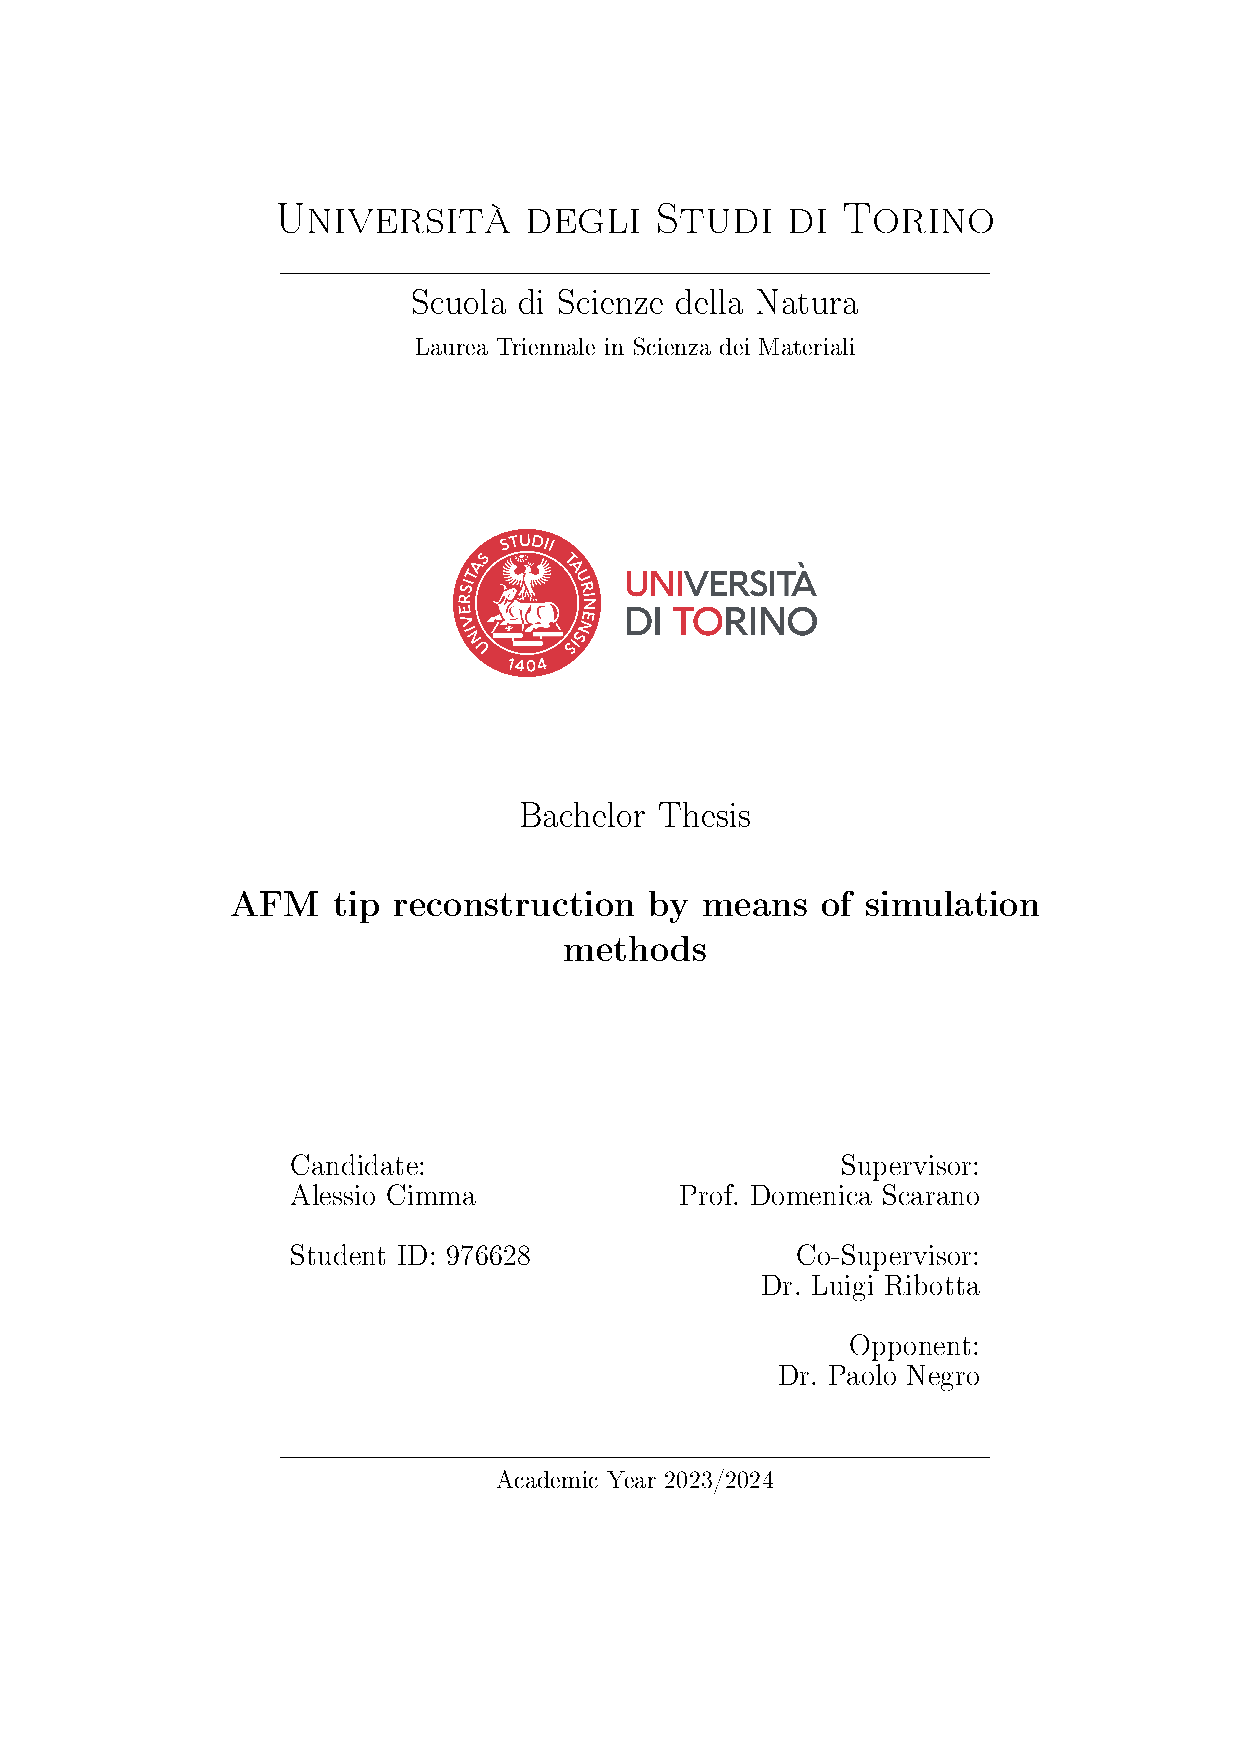
\includepdf[pages={1}]{./frontespizio.pdf}

% personale
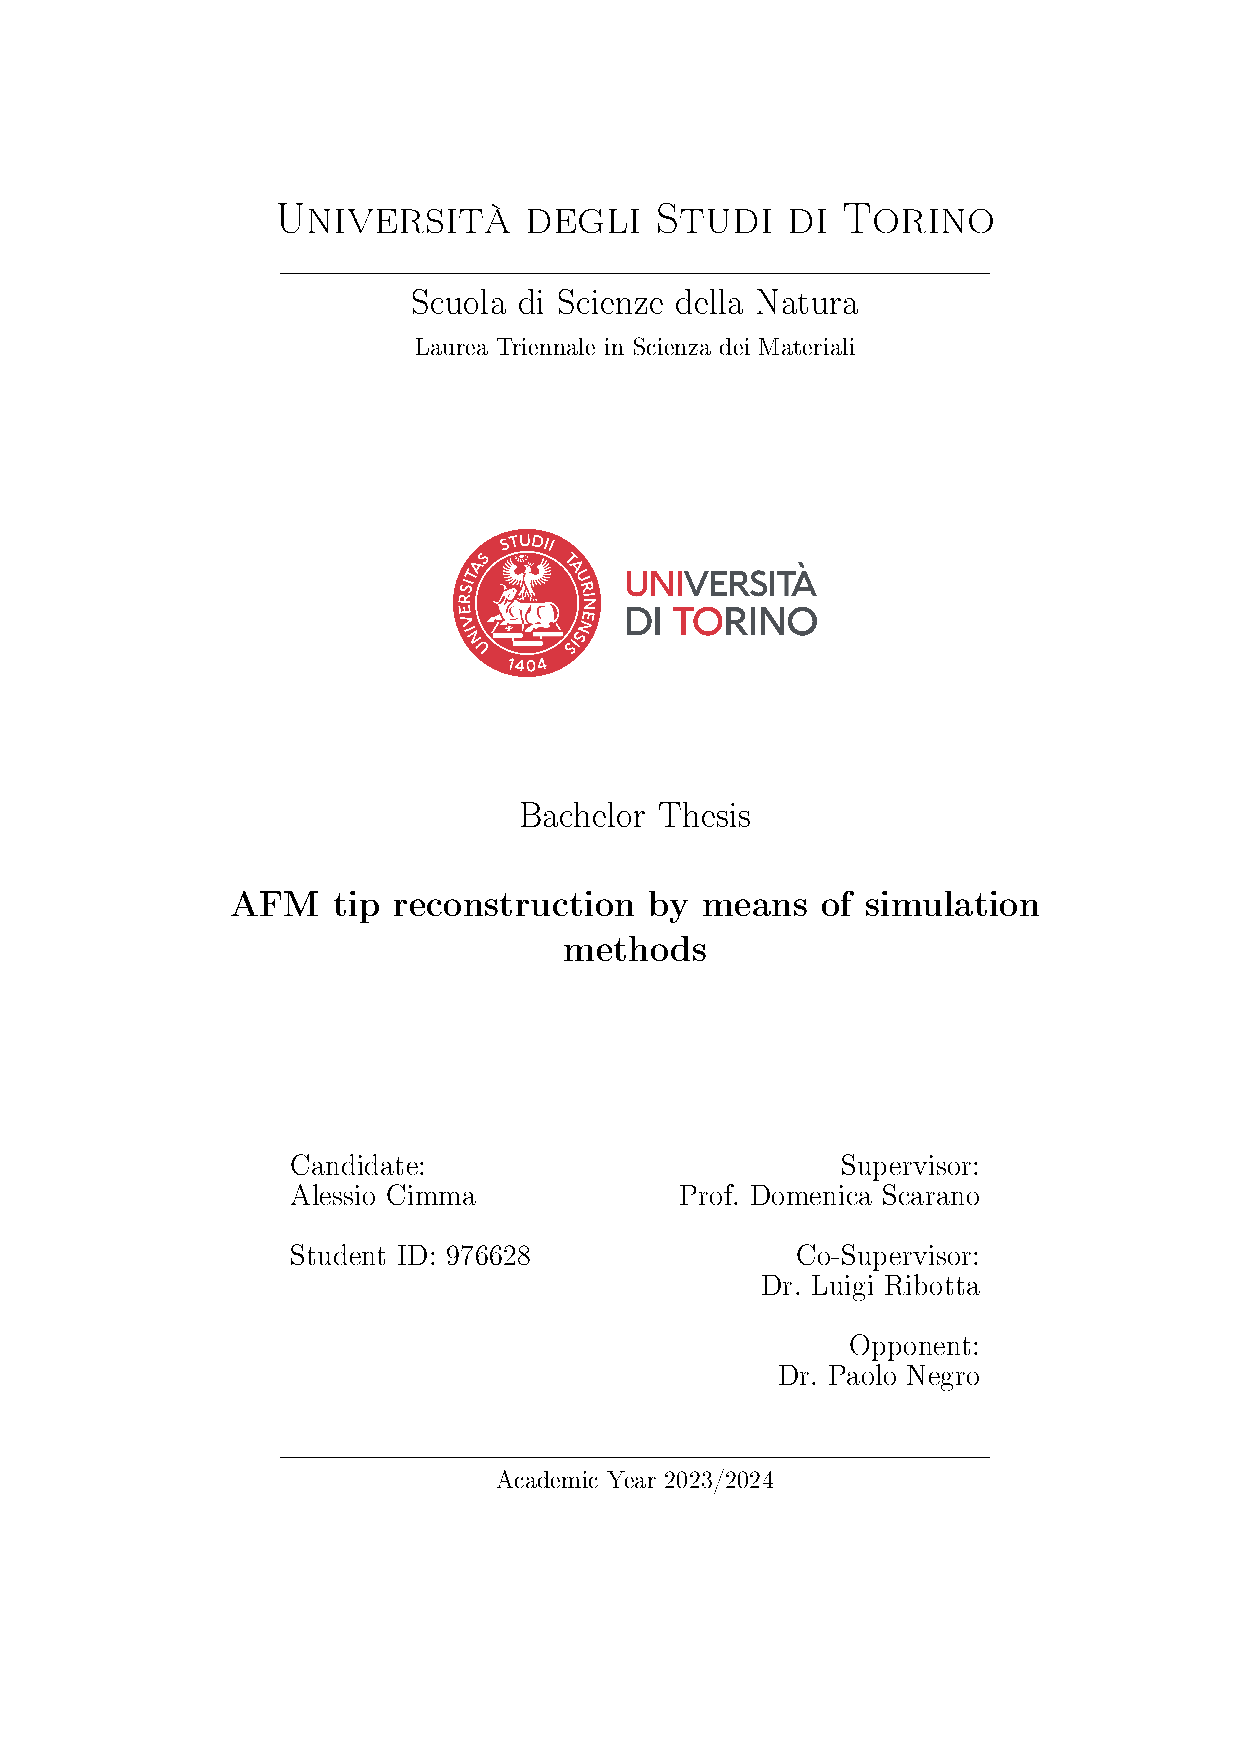
\includepdf[pages={1,2}]{./frontespizio.pdf}

\newpage

\section*{Acknowledgements}

\noindent This work has been made possible thanks to Andrea Giura, the first to embrace my unconventional ideas and have faith in my ability to bring this project to life.
\vspace{10pt}

\noindent I am deeply grateful to Prof.ssa Domenica Scarano for her invaluable guidance throughout this incredible journey.
\vspace{10pt}

\noindent Heartfelt thanks also go to the wonderful people at INRiM who supported me and made me feel part of a team. Special appreciation is to Dr. Luigi Ribotta for teaching me how to correctly approach such a difficult job and for helping me to express myself, to Jessica Petiti for helping me improve my hands-on skills in the lab, and to Sabrina Caria, whose constant positivity brightened the office.
\vspace{10pt}

\noindent I would also like to thank Francesca Capellino, who supported me over the past three years and kept me focused on my studies. Without her, I might still be preparing for some exams.

\pagenumbering{Roman}
\setcounter{page}{0}
\tableofcontents

\pagenumbering{arabic}
\setcounter{page}{0}
\newpage

\chapter{Introduction}

\section{Overview}

Nanometrology covers a wide range of techniques for the characterization and measurement of different kinds of materials at the nanometric scale. Atomic Force Microscope (AFM) is a widely used technique to measure 3D topographies at the nanoscale. The obtained AFM images are the results of the interaction of the sample with the tip.

The AFM techniques can achieve sub-nanometer resolution and accuracy along z direction (height measurements). On the contrary, the AFM lateral resolution (x and y directions) is strongly affected by the tip shape contribution. For this reason, a preliminar tip reconstruction before the data analysis is crucial. Nowadays, several AFM tip reconstruction methods are shown in literature, that are based on two main approaches for in situ characterisation, \textit{i.e.} the \textit{blind reconstruction} and the \textit{known tip characteriser techniques}.

\paragraph{Blind reconstruction:} the sample measured has a very rough surface (tip check) and no prior knowledge is required to perform the algorithm proposed by Villarrubia in 1997 \cite{Villarrubia}. The idea is to reconstruct the tip based on the wide variety of slopes in the sample. These allow us to get an idea of how well the tip can resolve vertical structures, thus indirectly obtaining the smallest possible shape that will contain the real tip.


\paragraph{Known tip characteriser:} the sample measured is a nanostructure with well-known dimensional parameters, that are then used in the reconstruction algorithm \cite{ribotta3}. Using a morphological filter, as further explained in section [9], we can trace the movement of a geometric object in space as if it rolled beneath a given surface. The obtained movement can be combined into a single object that is the actual shape of the real AFM tip. This explains why it is very important to have a faithful reconstruction of the nanostructure.


\section{Objective}

The known tip characteriser will be the approach studied in this work. In particular, we generalize the geometrical approach for the tip shape reconstruction method presented by Ribotta \textit{et al.} \cite{ribotta1,ribotta2,other_morphological} to any ideal structure, and we implement routines for the procedural generation of height maps with multiple tip characterisers. Our goal is to create a Python module that helps generating the ideal topography of the tip characteriser and, consequently, allows to reconstruct the tip shape by "eroding" the real measurement with the generated structure.

\vspace{10pt}

Fast and reliable generation of this ideal sample is not trivial and cannot be easily done by mathematic modelling of the nanostructures. The \textit{ray traced} approach allows to generate multiple models of the expected size and orientation and, consequently, to analyze them by means of image recognition algorithm. Finally, this allows to proceed with the eroding algorithm.

\chapter{The AFM}

\section{Overview}

Atomic force microscopy (AFM) is a technique that allows the 3D characterization of many types of samples (conductive, insulators, inorganic, organic, biological, etc.) and operates in air or liquid phase. Given its versatility, AFM can be coupled with other techniques by using specialized hardware and types of probes (e.g., scanning thermal microscopy, Kelvin probe force microscopy, infrared nanospectroscopy, etc). AFM, including various hyphenated techniques, permit analysis in various fields, such as polymer chemistry and physics, surface chemistry, cell biology, semiconductor science, and metrology.

The AFM topography results from the dilation of the sample shape, probe shape, and tip-sample-substrate interactions. An AFM image is commonly referred to as a 3D representation, although it is more referred to as a 2.5D reconstruction. The topography is a mapping of the heights given by a 2D array of numbers, which corresponds to the deflection of the cantilever as the tip scans the sample surface. Therefore, a not complete 3D reconstruction of the exposed surface is obtained, albeit limited by the tip geometry. In fact, it does not consider the portion of the sample in contact with the substrate. \cite{ribotta3}

The core of an AFM is its head, where the cantilever is located, which has the tip at its end. To scan the sample we drag a probe, known as the AFM tip, across it and register its elevation. Whenever the tip encounters an obstacle, it tries to match its height and to overcome it. The change of height is registered by the AFM using a laser-mirror system that converts the height displacement into an electric signal as shown in Fig. \ref{fig:AFM}.

\newpage

\begin{figure}[h]
    \centering
    % schema_afm
    \includegraphics[width=.6\textwidth]{./immagini/_power_afm4.png}
    \caption{AFM working principle}
    \label{fig:AFM}
\end{figure}

\section{Operational modes}

The AFM can operate in 3 different ways: contact mode, non-contact mode and tapping, based on the force region the AFM operates as shown in Fig. \ref{fig:AFM_modes_a}:
\begin{itemize}
    \item Contact mode: the deflection of the cantilever, proportional to the tip-sample
    interaction forces, provides sample topography.
    \item Non-contact mode: the vibration of cantilever at its resonance frequency is modified in amplitude and phase, due the interaction forces. To generate the images obtained in this work, the amplitude modulation was used, which gives not only topographic information, but also provides a feedback to keep the tip-sample distance constant (See Fig. \ref{fig:AFM_modes_b}).
    \item Tapping: the oscillation of the cantilever allows the tip to contact the sample cyclically, hence the force required to detach the tip from the sample is applied.
\end{itemize}

\newpage

\begin{figure}[h]
    \centering
    % schema_afm
    \includegraphics[width=0.95\textwidth]{./immagini/_power_afm3.png}
    \caption{Force region of operability}
    \label{fig:AFM_modes_a}
\end{figure}

\begin{figure}[h]
    \centering
    % schema_afm
    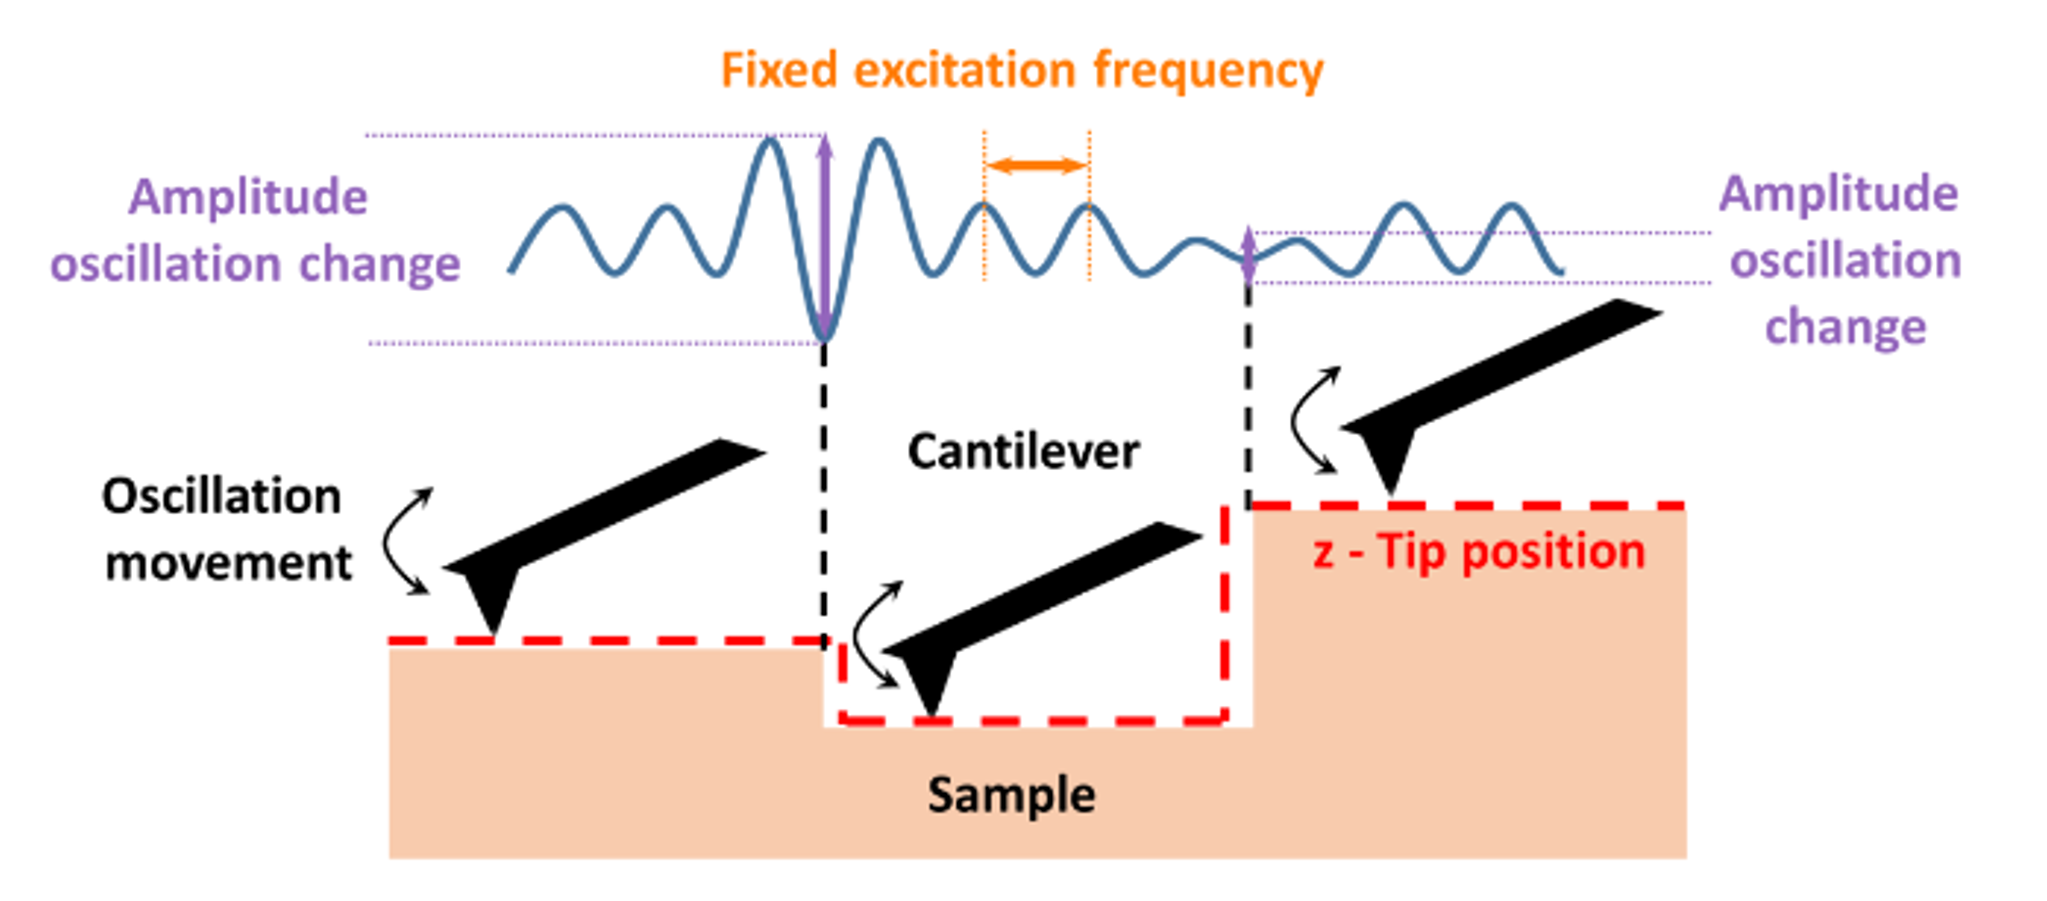
\includegraphics[width=.8\textwidth]{./immagini/non_contact_mode.png}
    \caption{Sketch of an AFM cantilever operating in non-contact mode (amplitude modulation) \cite{immagine_luigi}}
    \label{fig:AFM_modes_b}
\end{figure}

% \begin{figure}[ht]
%     \centering
%     \begin{subfigure}[b]{0.48\textwidth}
%         % forces
%         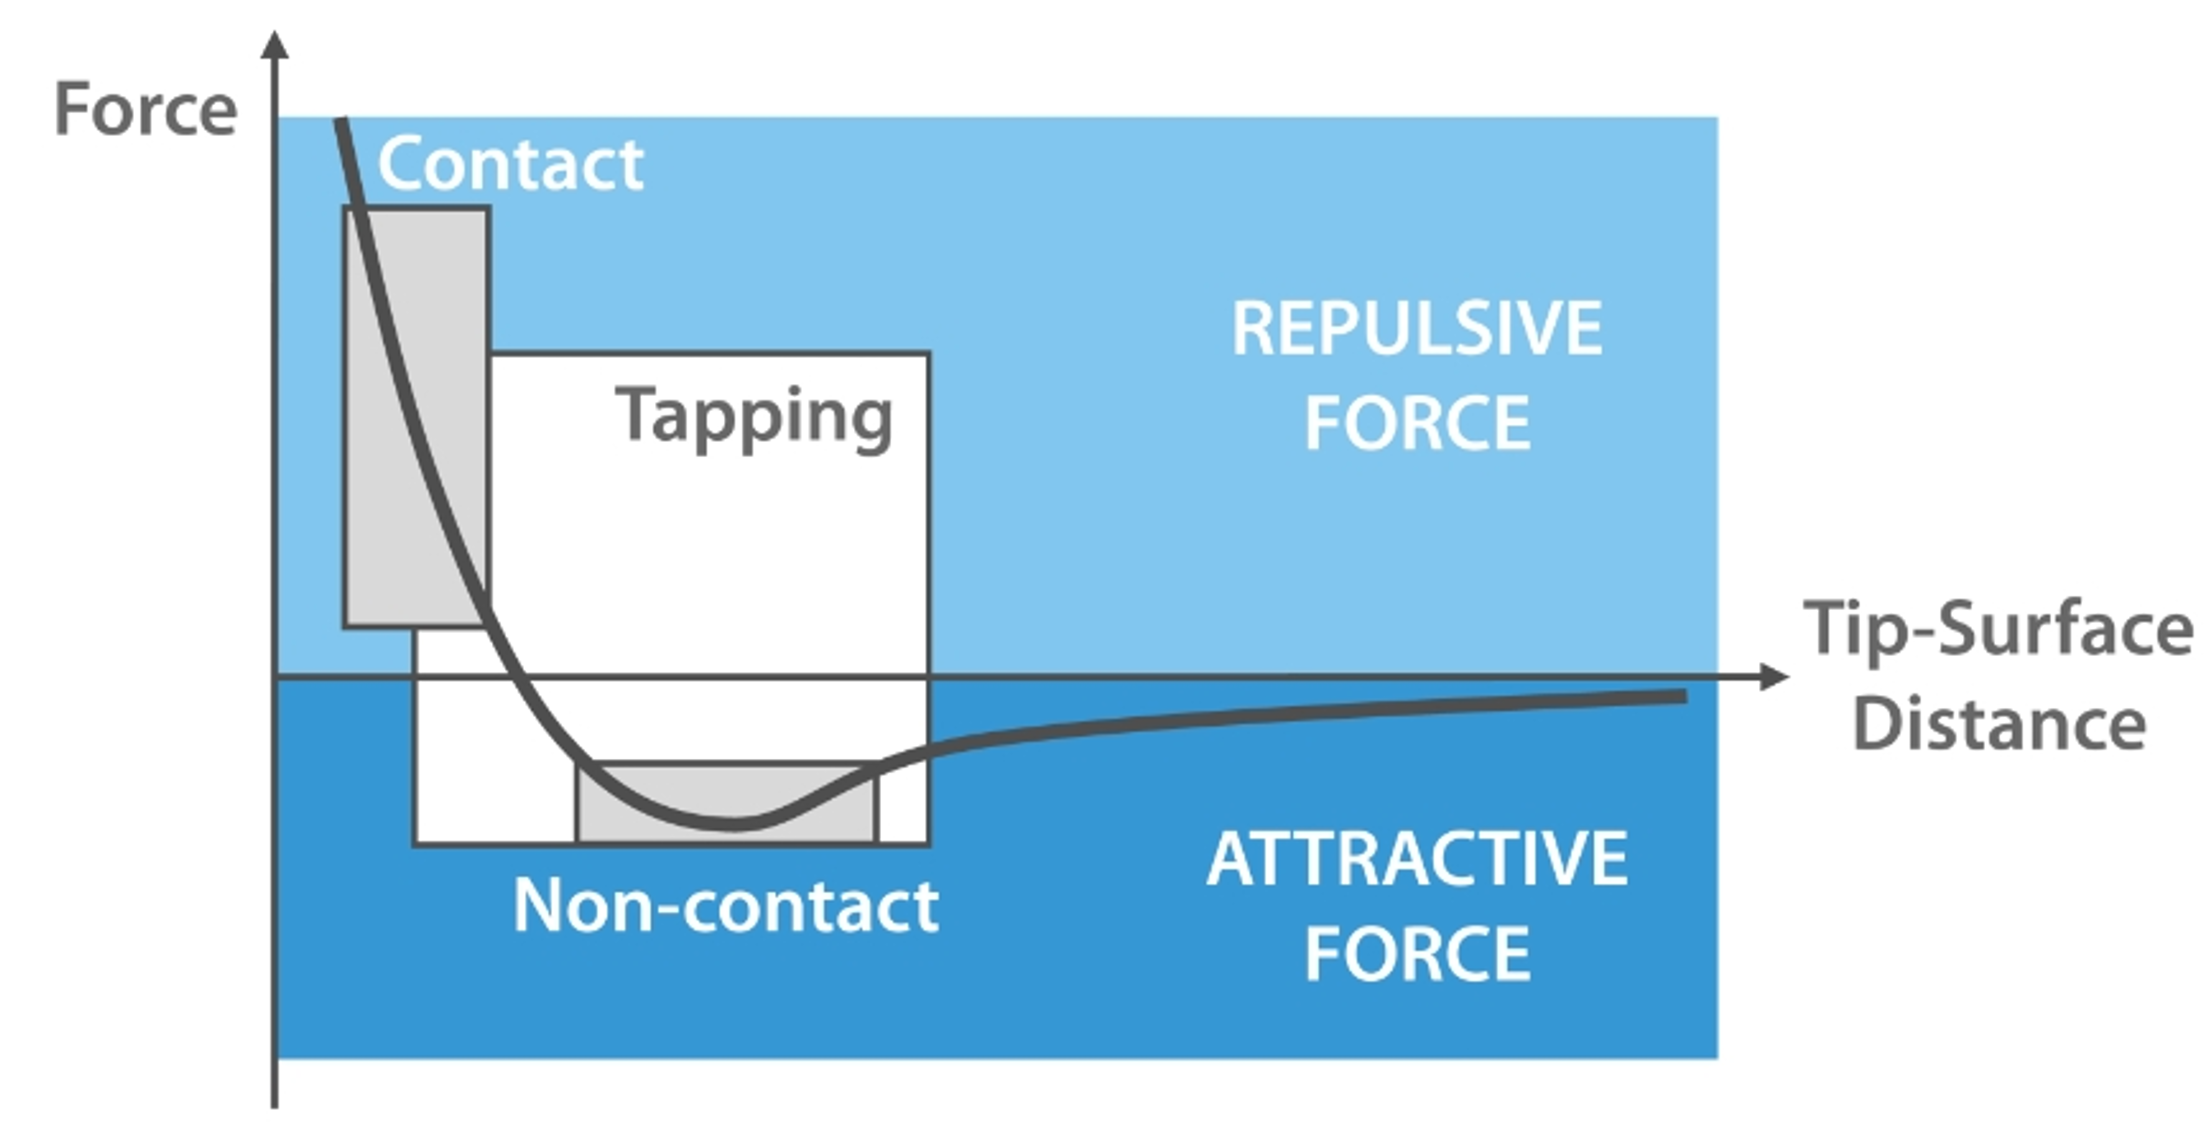
\includegraphics[width=.98\textwidth]{./immagini/forces.png}
%         \caption{}
%         \label{fig:AFM_modes_a}
%     \end{subfigure}
%     \hfill
%     \begin{subfigure}[b]{0.48\textwidth}
%         % non_contact_mode
%         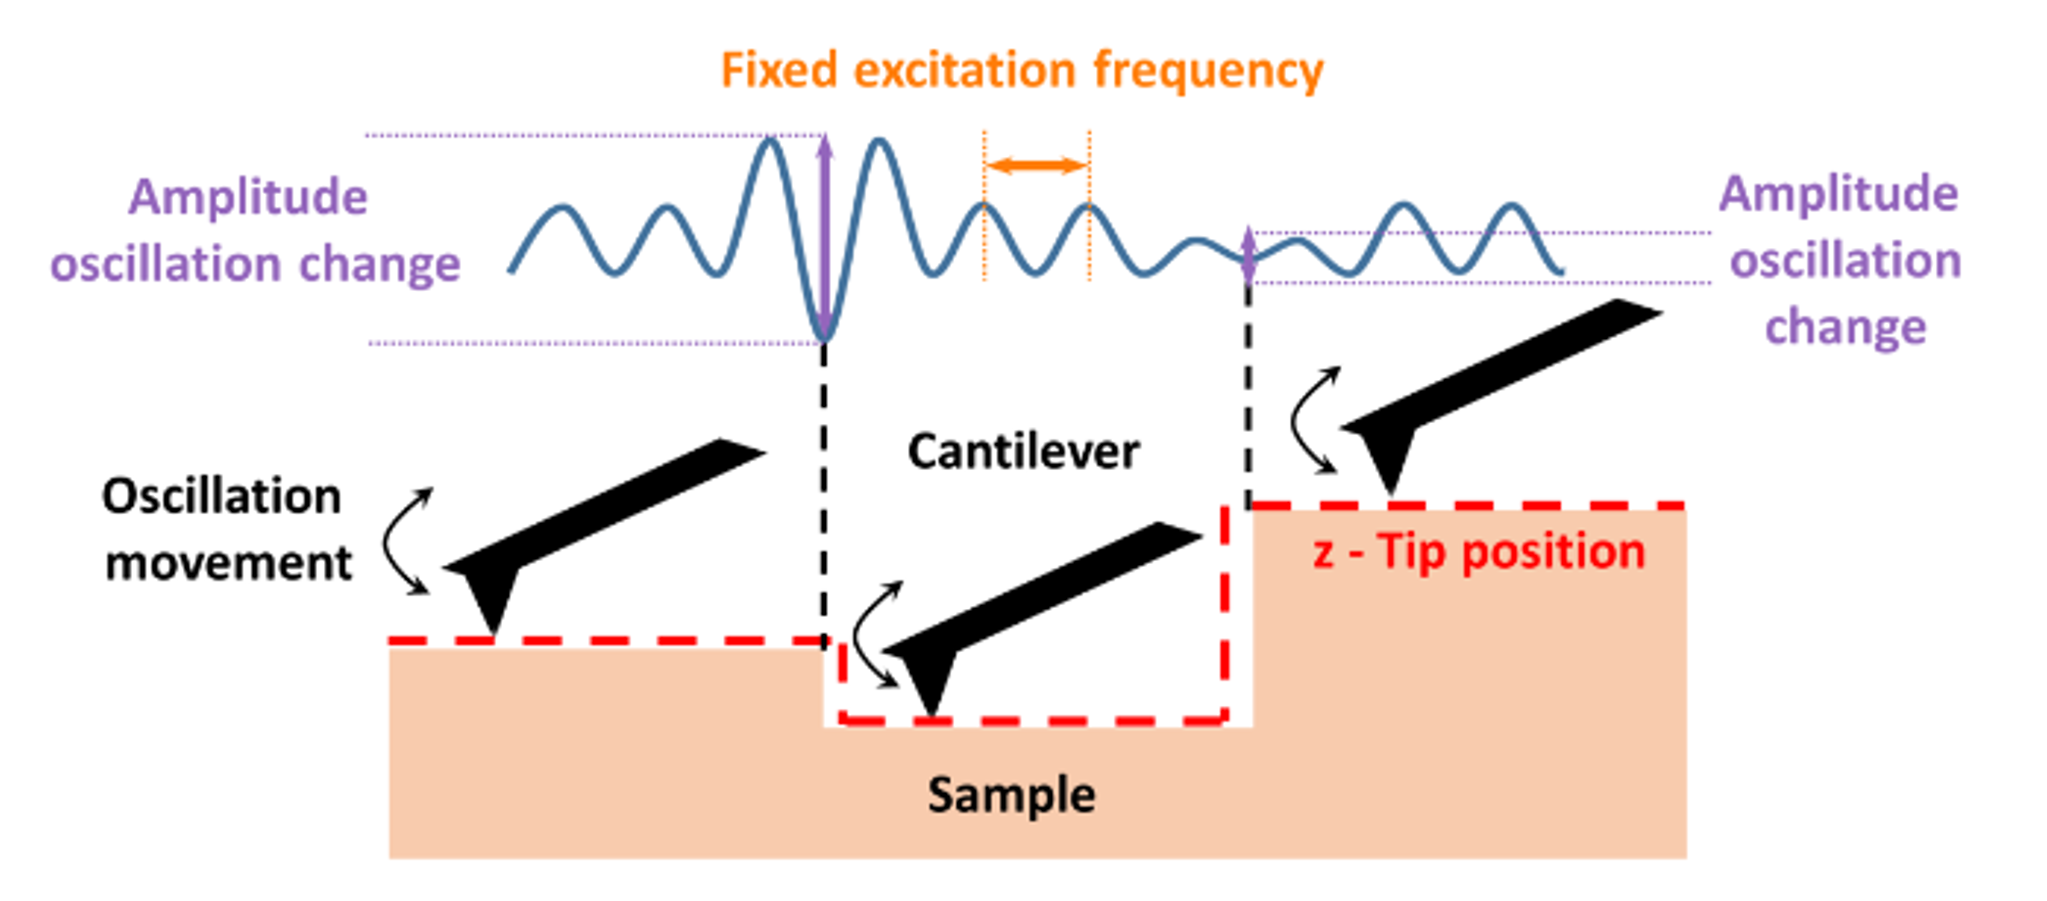
\includegraphics[width=.98\textwidth]{./immagini/non_contact_mode.png}
%         \caption{}
%         \label{fig:AFM_modes_b}
%     \end{subfigure}
%     \caption{a) Force region of operability b) Sketch of an AFM cantilever operating in non-contact mode (amplitude modulation) \cite{immagine_luigi}}
%     \label{fig:AFM_modes}
% \end{figure}

In this work, we focus on improving the lateral resolution of the AFM image, by removing the interference of the tip from the topography. It is known that the tip has an actual physical size, that deteriorates the lateral resolution. In fact, the quality of the lateral resolution is given by the tip-sample interaction and by the pixel size. Tip-sample and tip-substrate interactions refer to elasticity, whereas sample-substrate deformation refers to plasticity. 
    
The specific AFM used to generate these images is a custom made metrologic AFM, where everything except the head (obtained from Bruker) was designed and built at INRiM labs. This was achieved by building around the AFM a set of 3 interferometers, one along each axis, which guarantees the direct traceability to the SI (The International System of Units). The used tip $\mu$Masch (NSC-AlBS-14) \cite{ribotta3} works in non-contact mode.

\chapter{Structure generation}

\section{Chosen approach}

In order to reconstruct the tip shape via ray tracer method, which is an innovative way to simulate and reconstruct the tip, an ideal image of the measured sample has been generated. To this purpose, an ideal point-shaped tip has been considered and approximated by means of a monoatomic tip or a Dirac's delta shaped tip. Thus, the simulation of the ideal measurement has been performed by computing the height of each pixel by using \textit{z-test} (or \textit{depth-test}) technique \cite{raycasting_ztest}, that is commonly used in ray tracers. In particular, \textit{z-test} relies on testing the distance between a given point and the planar camera and, if another point that should be drawn in the same pixel is closer, the algorithm substitutes the previous one. (see Fig. \ref{fig:concept}). This will ensure a correct occlusion handling.

\begin{figure}[ht]
    \centering
    %  concept
    \includegraphics[width=.95\textwidth]{./immagini/concept.png}
    \caption{Ray Tracer z-test method}
    \label{fig:concept}
\end{figure}

\newpage

The constant evolution in terms of performances, due to ever-improving hardware and dedicated programming languages, makes raytracers advantageous \cite{GPU_language}. In fact, the field of ray tracing has made significant progress in recent years, with improvements in rendering speed, accuracy, and efficiency, largely driven by the use of powerful graphics processing units (GPUs). The ability to simulate ideal measurements and accurately reconstruct tip shapes using ray tracing techniques opens up new possibilities for improving the precision and speed of tip reconstruction algorithms in AFM studies.

\section{Models and nanoparticles}

The general method used to create different structures is based on the generation of meshes made of triangles using some known dimensional parameters. Besides z-test, ray tracers usually will perform other shader calculation in order to create photorealistic images. For this project, we will borrow just the algorithm for correctly rendering triangles and their occlusions \cite{raytracer1,raytracer2}.

\vspace{10pt}

Since the coordinates of the mesh triangles are known \textit{a priori}, we can further speed up the calculations by employing a technique called rasterization and fragment processing. This technique calculates the height at a specific point from an interpolation of the three vertices of the triangle in which the point is enclosed using its barycentric coordinates \cite{rasterization}.

\vspace{10pt}

We can create a standard and normalized model of each structure we want to study (spheres, cubes, steps, etc.) with open source or external 3D modelling programs (e.g. Blender \cite{blender}). Hence, given an input of parameters, we can generate the model of the correct size, orientation and position using scale, rotation and traslation matrices. In this way, we can generate an array of triangles that will be resulting in the ideal structure, composed of multiple nanoparticles without resorting to mathematical modelling of the surface.

\vspace{10pt}

In the following sections we will explain all the steps needed to perform the operations starting from the triangle meshes to obtain the final ideal topography.
It is worth knowing that this work focuses on the union of two very broad and different fields. In the future, there will be the possibility to generate the mesh from scratch, while for now, we begin our studies from pre-calculated models. Future routines will also be able to adapt and generate models for more complex geometries and from a base set of written instructions.

\newpage

\section{Triangles}

\paragraph{Barycentric coordinates: }

Every single model that will be generated and simulated will be structured from triangles. This means that we can extract various attributes using barycentric coordinates as shown in Fig. \ref{fig:bary_a} and \ref{fig:bary_b}. Using this method we can define an information of interest (such as depth) at the vertices and interpolate them to obtain a smooth final image as shown in Fig. \ref{fig:bary_b}.

\begin{figure}[ht]
    \centering
    \begin{subfigure}[b]{0.45\textwidth}
        % bary1
        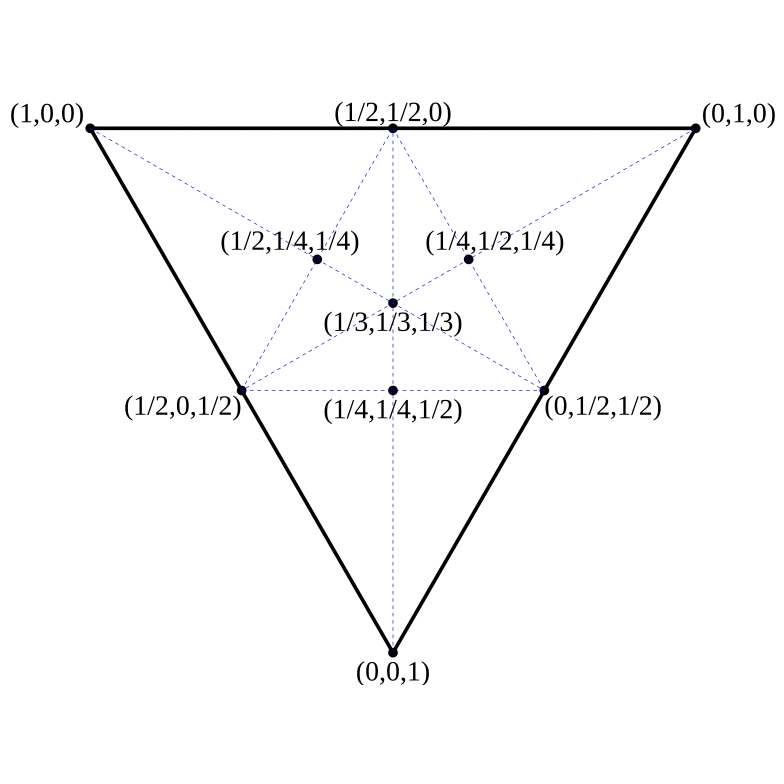
\includegraphics[width=.95\textwidth]{./immagini/bary1.png}
        \caption{}
        \label{fig:bary_a}
    \end{subfigure}
    \hfill
    \begin{subfigure}[b]{0.45\textwidth}
        % bary2
        \includegraphics[width=.95\textwidth]{./immagini/bary2.png}
        \caption{}
        \label{fig:bary_b}
    \end{subfigure}
    \caption{a) Geometrical construction, b) smooth interpolation of baricentric coordinates}
    \label{fig:bary}
\end{figure}

Notice that this process is applied to each triangle that composes the model, thus leading to a heavy computation very quickly. In this case the parallelised computation of powerful graphics processing units (GPUs) proves useful.

\paragraph{Depth test and overalapping:} Once we have more than one triangle there might be overlapping, and to address this issue, we use a ray-tracer simulating technique to test how far a triangle is respect to the camera. In this way we can correctly identify which triangle should actually be part of the simulated nanostructure, see Fig. \ref{fig:depth}. This process will be speed up incredibly by using the standard graphical pipeline used in the video-games industry, backed up by the physical and mathematical correctness of the ray-tracer approach. 

\vspace{10pt}

Hence, by means of this method, we can correctly simulate the nanoparticles discussed in the following chapters.

\newpage

\begin{figure}[ht]
    \centering
    \begin{subfigure}[b]{0.32\textwidth}
        % depth
        \includegraphics[width=.95\textwidth]{./immagini/depth.png}
        \caption{}
        \label{fig:depth_a}
    \end{subfigure}
    \hfill
    \begin{subfigure}[b]{0.32\textwidth}
        % depth2
        \includegraphics[width=.95\textwidth]{./immagini/depth2.png}
        \caption{}
        \label{fig:depth_b}
    \end{subfigure}
    \hfill
    \begin{subfigure}[b]{0.32\textwidth}
        % depth3
        
\includegraphics[width=.95\textwidth]{./immagini/depth3.png}
        \caption{}
        \label{fig:depth_c}
    \end{subfigure}
    \caption{a) A pair of triangles of unknown Z height b) Zoom of the overlapping surface c) Final result, obtained from comparing the depth at which each pixel is located}
    \label{fig:depth}
\end{figure}

\section{Spheres}

The standard model is created in Blender using an icosphere with 5 subdivisions. It is centred in the origin with radius r equal to 1.
Then, it is translated by a vector v = (x, y, z) to it is new position and scaled of a given factor in order to match the desired position and dimension. The z-traslation equals to r/2, in order to place the base of the sphere on the floor. This ensures that the nanoparticle rests perfectly on the substrate.
Some examples of generated images are reported in Fig. \ref{fig:sphere}a-c. In particular, Fig. \ref{fig:sphere_b} and \ref{fig:sphere_c} show also compenetrated spheres that are successfully handled by this system.

\begin{figure}[ht]
    \centering
    \begin{subfigure}[b]{0.32\textwidth}
        % sfera_singola
        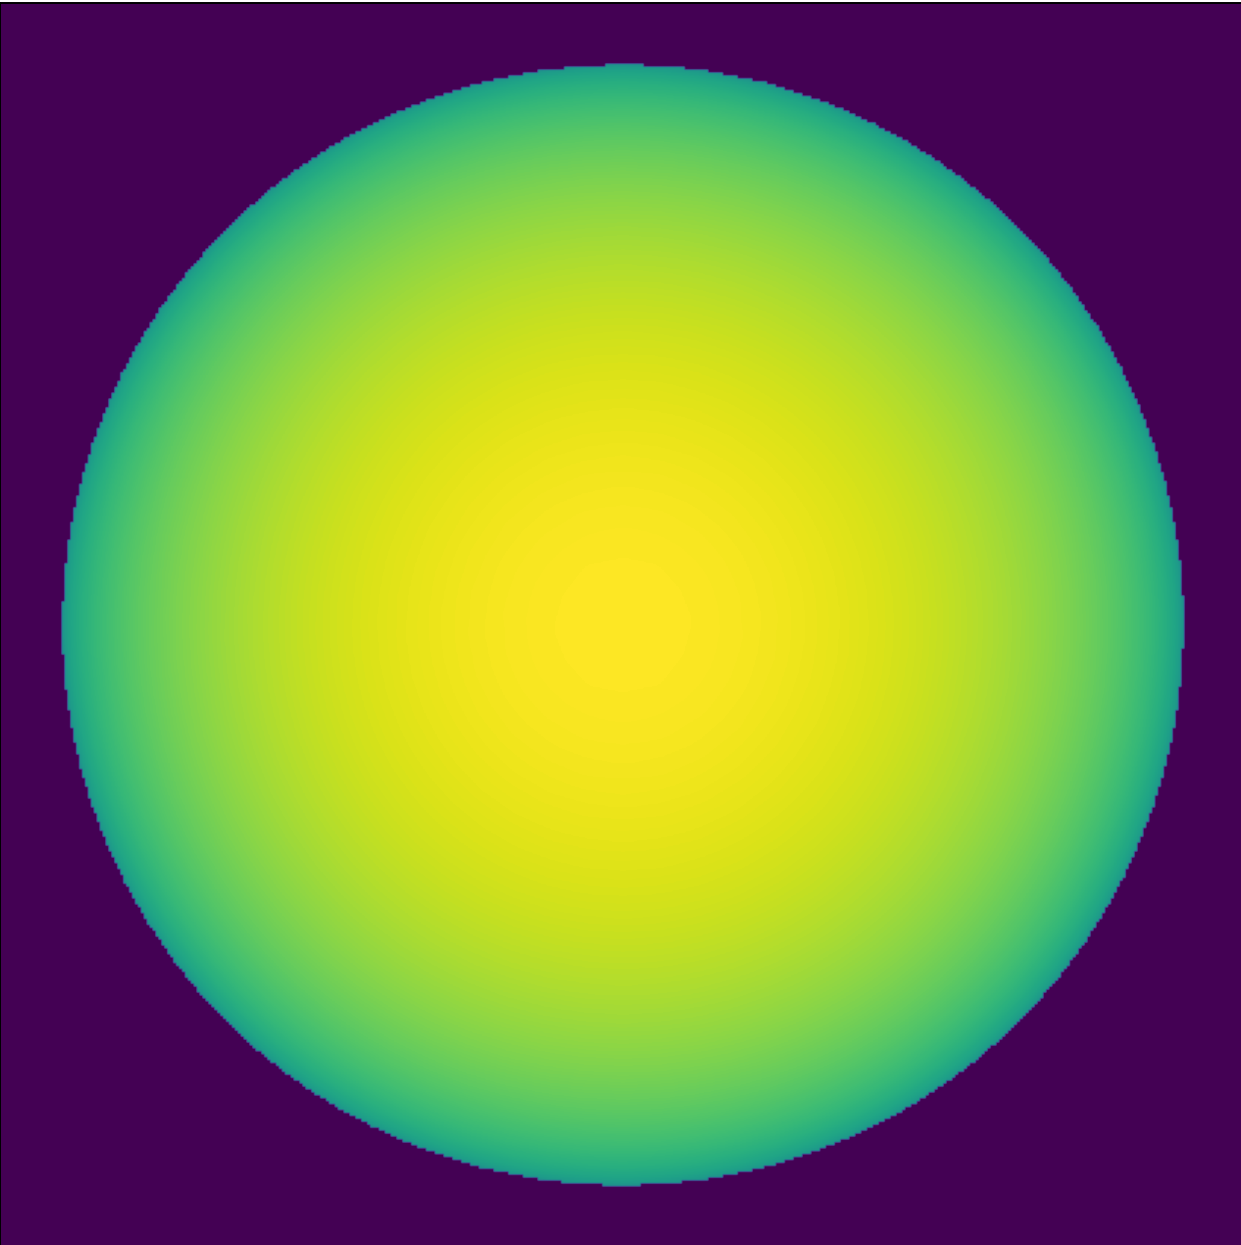
\includegraphics[width=.95\textwidth]{./immagini/sfera_singola.png}
        \caption{}
        \label{fig:sphere_a}
    \end{subfigure}
    \hfill
    \begin{subfigure}[b]{0.32\textwidth}
        % sfera_doppia
        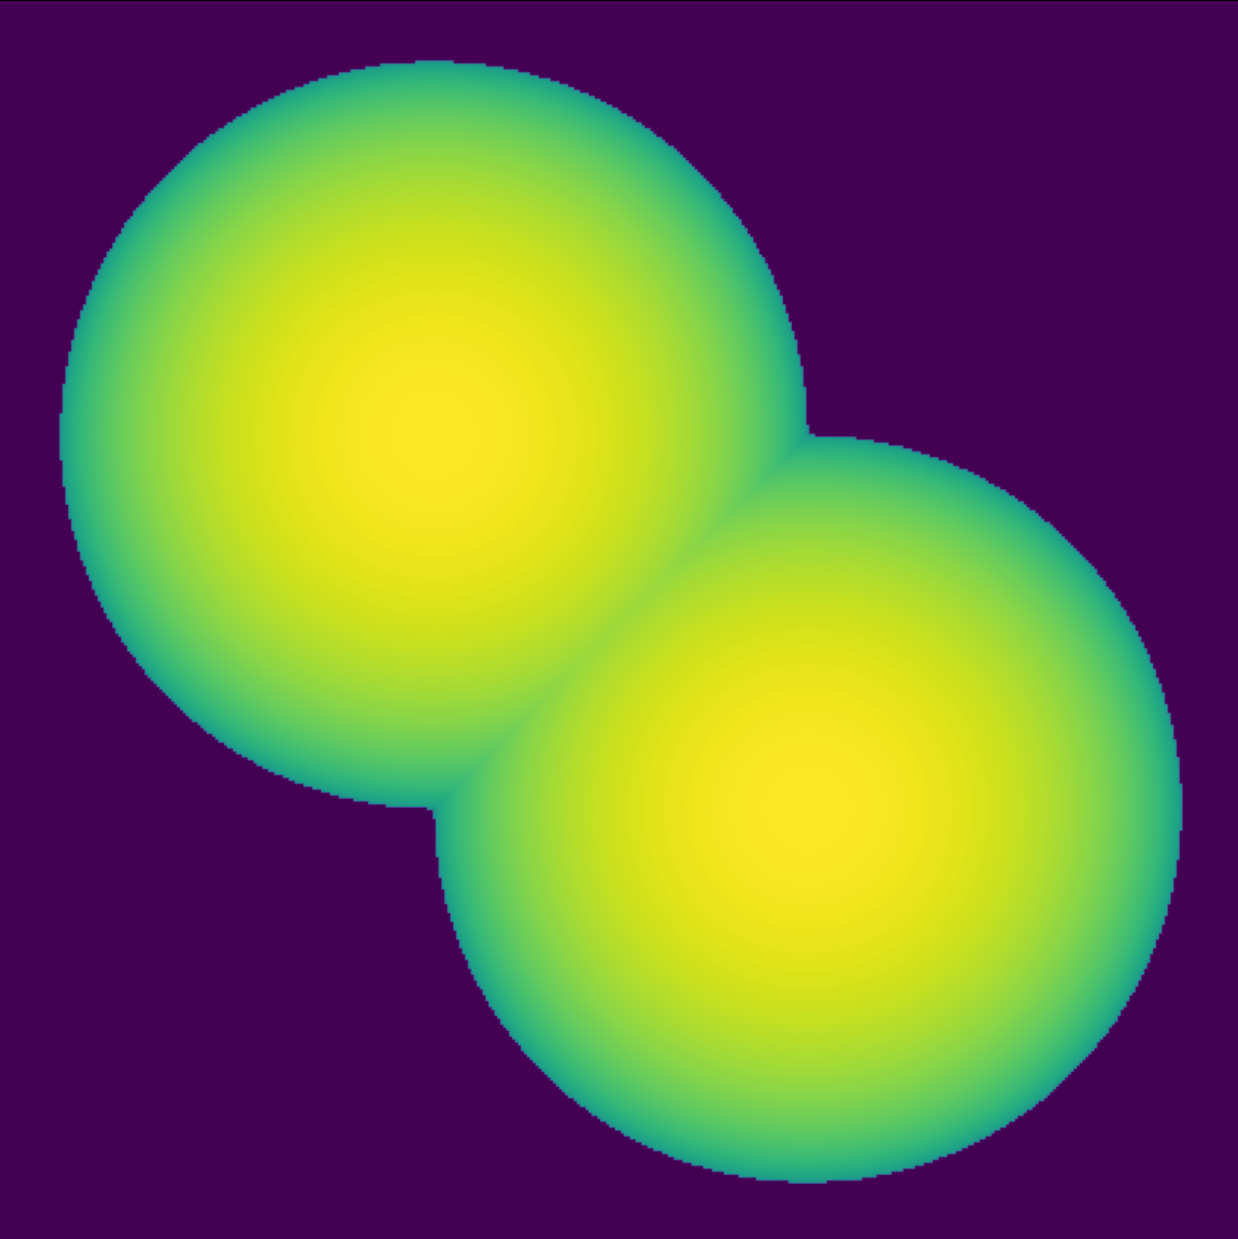
\includegraphics[width=.95\textwidth]{./immagini/sfera_doppia.png}
        \caption{}
        \label{fig:sphere_b}
    \end{subfigure}
    \hfill
    \begin{subfigure}[b]{0.32\textwidth}
        % sfera_statistica
        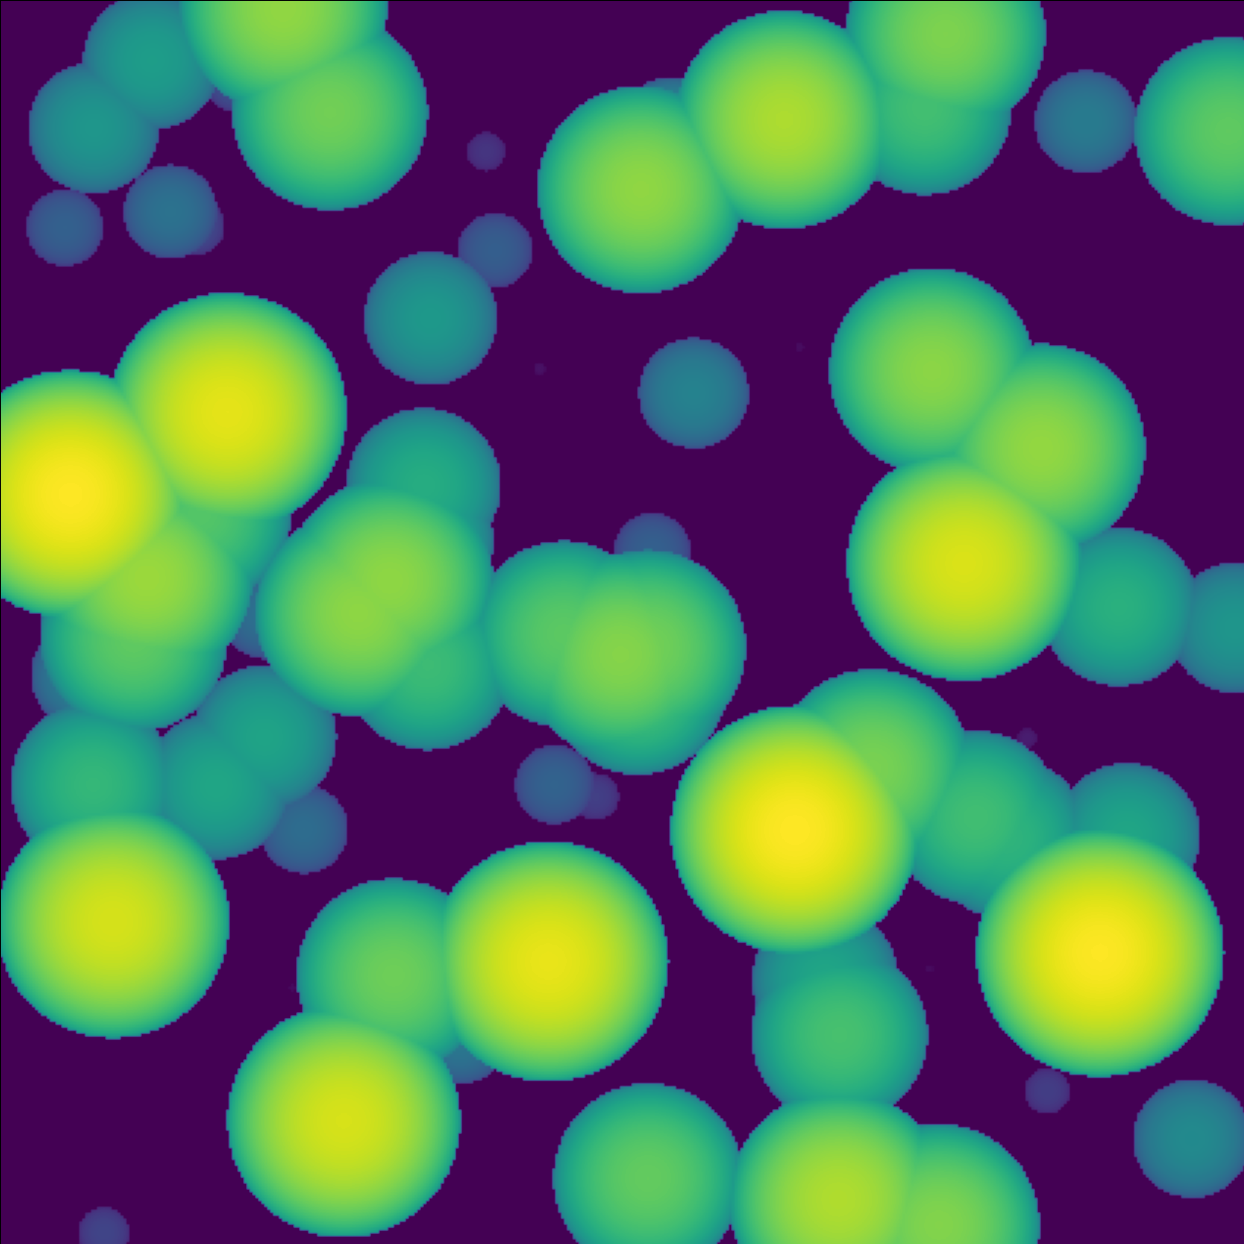
\includegraphics[width=.95\textwidth]{./immagini/sfera_statistica.png}
        \caption{}
        \label{fig:sphere_c}
    \end{subfigure}
    \caption{a) Single, b) Double and  c) Statistic used spheres}
    \label{fig:sphere}
\end{figure}

\newpage

\section{Nanosheets}

\paragraph{Creation process: }

The standard model is created in Blender using a cube with a central subdivision along the Y axis. It is centred in the origin with half size equal to 1. The geometrical shape of a nanosheet is well defined \cite{angleTIO2} with an angle of 68.3° obtained from anatase $TiO_2$ X-ray measurements. This recurring feature gives us the possibility to generate a standard, unitary-sized, model to use as a template for all the future instances.
The final model is obtained after a series of steps applied to the template model, as shown in Fig. \ref{fig:nano_creation}:
%
\begin{itemize}
    \item Scale along Y axis (to match the correct ratio between height and width) equals to: $S_Y = h / w$
    \item Scale along XZ plane (to generate the insets of the superior and inferior faces) equals to: $S_{XZ} = 1 - (h_{\text{eff}} / tan(68.3^{\circ}))$
\end{itemize}
%
Where h\_eff is the new calculated height.

\begin{figure}[ht]
    \centering
    \begin{subfigure}[b]{0.3\textwidth}
        % nano_1_1
        \includegraphics[width=.95\textwidth]{./immagini/nano_1_1.png}
        \caption{}
        \label{fig:nano_creation_a}
    \end{subfigure}
    \hfill
    \begin{subfigure}[b]{0.3\textwidth}
        % nano_1_2
        \includegraphics[width=.95\textwidth]{./immagini/nano_1_2.png}
        \caption{}
        \label{fig:nano_creation_b}
    \end{subfigure}
    \hfill
    \begin{subfigure}[b]{0.3\textwidth}
        % nano_1_3
        \includegraphics[width=.95\textwidth]{./immagini/nano_1_3.png}
        \caption{}
        \label{fig:nano_creation_c}
    \end{subfigure}
    \caption{Creation of steps: a) Scale along Y axis, b) Inset of the superior and inferior surfaces c) Final standard model}
    \label{fig:nano_creation}
\end{figure}

\paragraph{Positioning process: }

The additional information provided enables us to execute additional steps. This will include passages such as: floor process, positioning, rotation and scale, as shown in Fig. \ref{fig:nano_pos}:


\begin{itemize}
    \item The standard model is centered in the world origin, this means that we need to floor it (position the model so it will not clip with the floor substrate).
    \item Given the different size of the particle can be scaled accordingly, remembering that the half size of the standard model is equal to 1. This means we need to scale everything by a factor of (nominal\_size / 2).
    \item Now that the particle is generated and resized it now possible to traslate it by a vector $\vec{v}$ = (x, z) on the floor.
\end{itemize}

\begin{figure}[ht]
    \centering
    \begin{subfigure}[b]{0.3\textwidth}
        % nano_2_1
        \includegraphics[width=.95\textwidth]{./immagini/nano_2_1.png}
        \caption{}
        \label{fig:nano_pos_a}
    \end{subfigure}
    \hfill
    \begin{subfigure}[b]{0.3\textwidth}
        % nano_2_2
        \includegraphics[width=.95\textwidth]{./immagini/nano_2_2.png}
        \caption{}
        \label{fig:nano_pos_b}
    \end{subfigure}
    \hfill
    \begin{subfigure}[b]{0.3\textwidth}
        % nano_2_3
        \includegraphics[width=.95\textwidth]{./immagini/nano_2_3.png}
        \caption{}
        \label{fig:nano_pos_c}
    \end{subfigure}
    \caption{Creation of steps: a) Scale along Y axis, b) Inset of the superior and inferior surfaces c) Final standard model}
    \label{fig:nano_pos}
\end{figure}

\newpage

\paragraph{Examples: }

Some examples of generated images are reported in Fig. \ref{fig:nanosheet}a-c. In particular, Fig. \ref{fig:nanosheet_b} and \ref{fig:nanosheet_c} show compenetrated nanosheets, that are successfully handled by this system.

\begin{figure}[ht]
    \centering
    \begin{subfigure}[b]{0.3\textwidth}
        % nanosheet_singola
        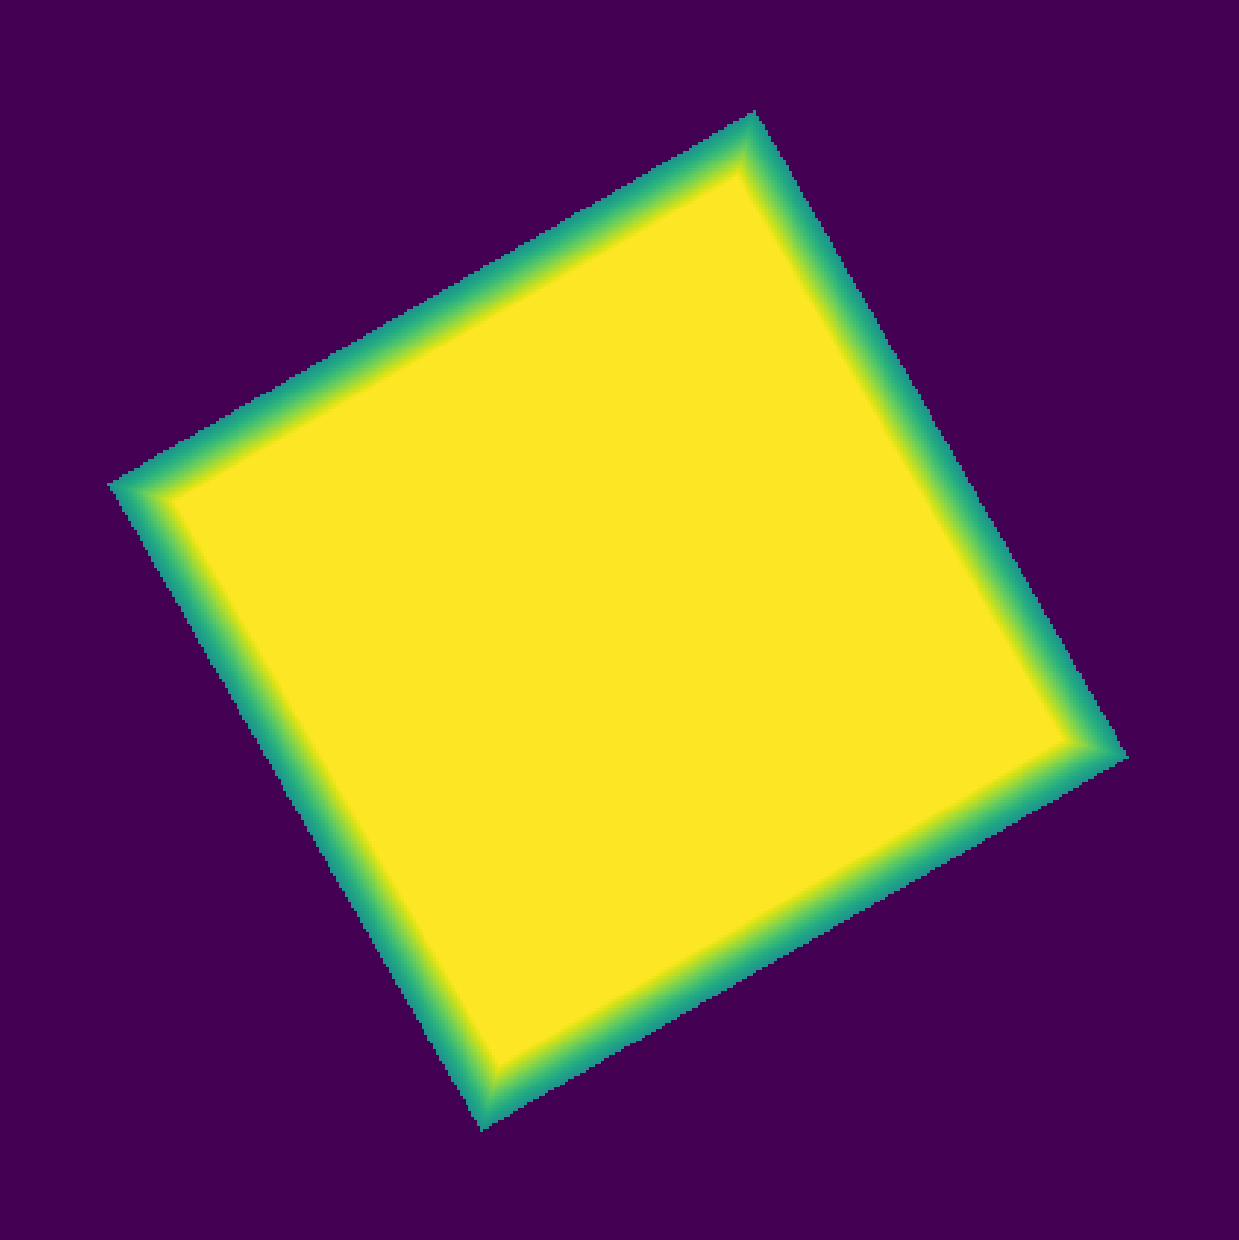
\includegraphics[width=.95\textwidth]{./immagini/nanosheet_singola.png}
        \caption{}
        \label{fig:nanosheet_a}
    \end{subfigure}
    \hfill
    \begin{subfigure}[b]{0.3\textwidth}
        % nanosheet_doppia
        
\includegraphics[width=.95\textwidth]{./immagini/nanosheet_doppia.png}
        \caption{}
        \label{fig:nanosheet_b}
    \end{subfigure}
    \hfill
    \begin{subfigure}[b]{0.3\textwidth}
        % nanosheet_statistica
        
\includegraphics[width=.95\textwidth]{./immagini/nanosheet_statistica.png}
        \caption{}
        \label{fig:nanosheet_c}
    \end{subfigure}
    \caption{a) Single, b) Double and  c) Statistic used nanosheets}
    \label{fig:nanosheet}
\end{figure}

\newpage

\section{Bipyramids}

\paragraph{Creation process: }

The whole process is very similar to the nanosheets one. The key difference is that the model becomes taller therefore more unstable. It will be necessary to lay the bipyramid down on one side. This is not a fixed rule, but statistically it's more common to find the nanoparticle on it's more stable equilibrium.

The standard model is created in Blender using a cube with a central subdivision along the Y axis. It is centered in the origin with half size equal to 1.

Several other passages are applied in order to obtain the correct model to use later, as shown in Fig. \ref{fig:bipyramids_process}:

\begin{itemize}
    \item Scale along Y axis (to match the correct ratio between height and width) equals to: $S_Y = h / w$
    \item Scale along XZ plane (to generate the insets of the superior and inferior faces) equals to: $S_{XZ} = 1 - (h_{eff} / tan(68.3^{\circ}))$
\end{itemize}

Where h\_eff is the new calculated height and $68.3^{\circ}$ is the crystalline angle of anatase $TiO_2$ from X-ray measurements.

\begin{figure}[ht]
    \centering
    \begin{subfigure}[b]{0.3\textwidth}
        % bipi_1_1
        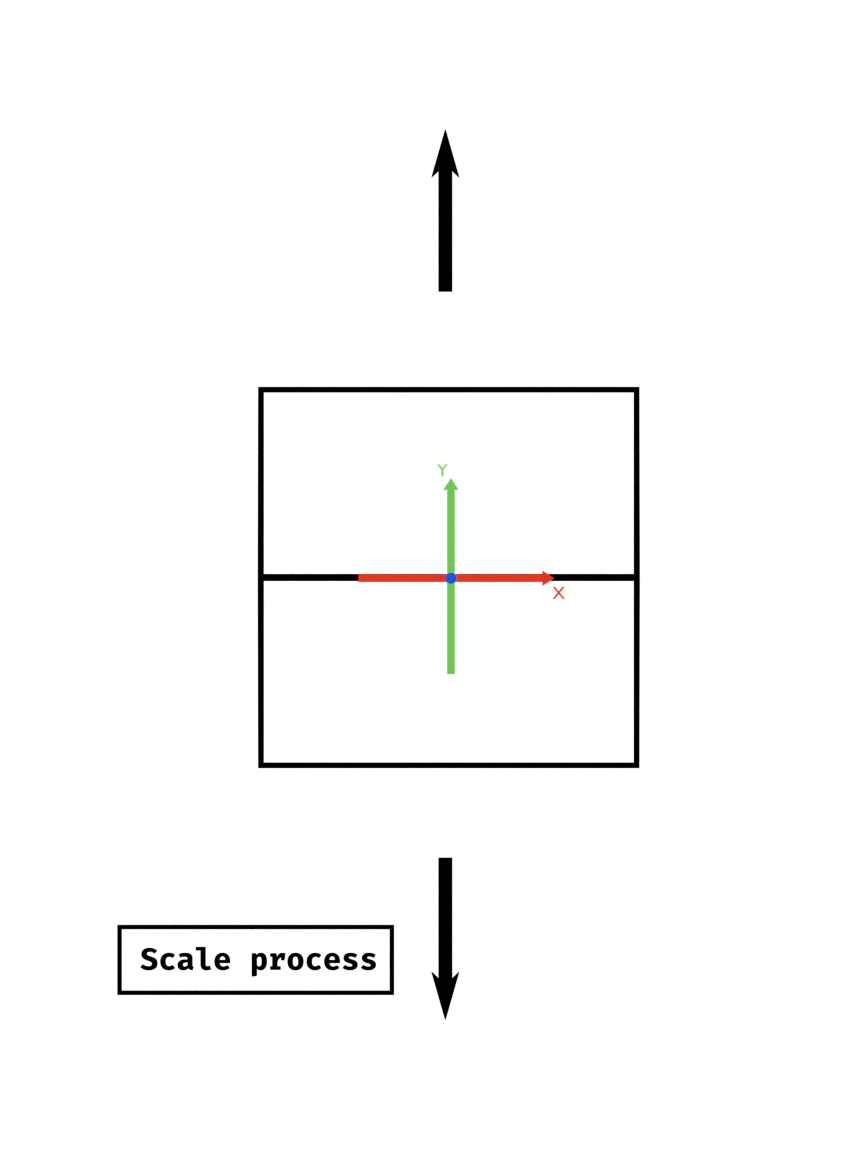
\includegraphics[width=.95\textwidth, clip]{./immagini/bipi_1_1.png}
        \caption{}
        \label{fig:bipyramids_process1}
    \end{subfigure}
    \hfill
    \begin{subfigure}[b]{0.3\textwidth}
        % bipi_1_2
        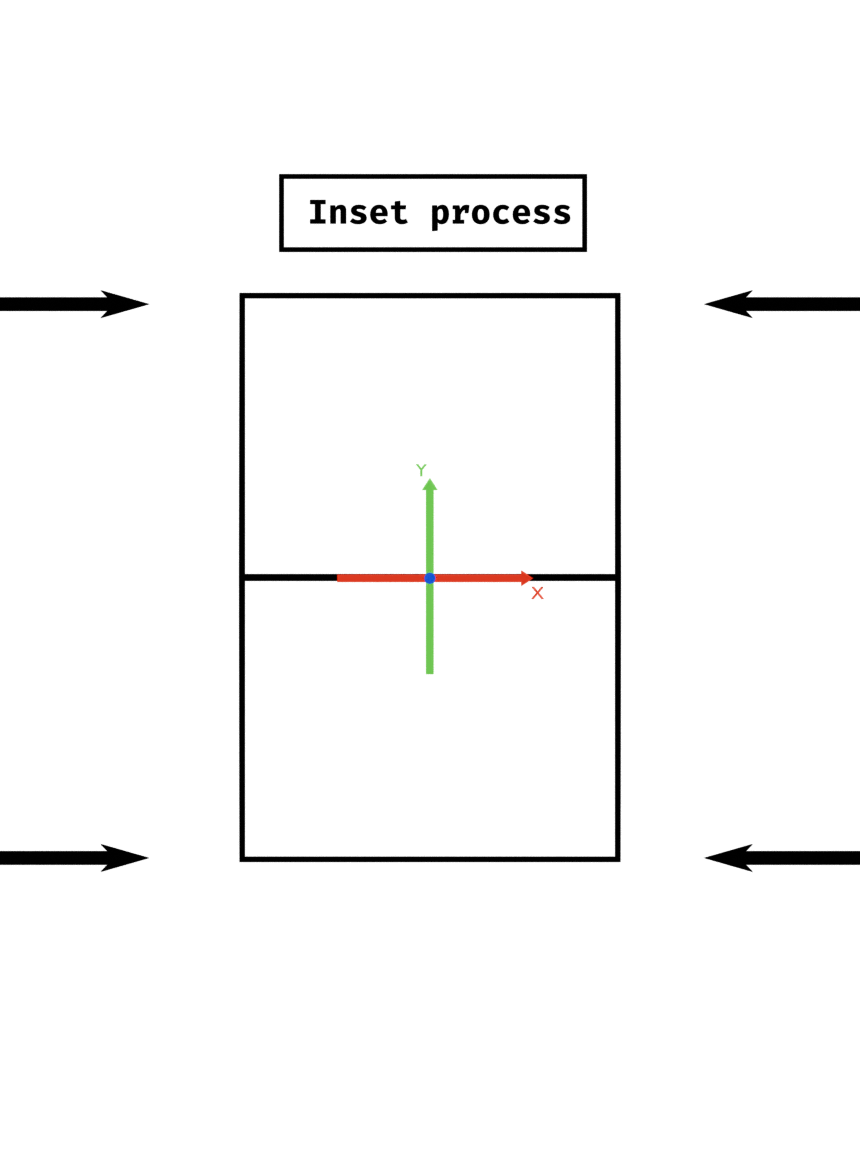
\includegraphics[width=.95\textwidth, clip]{./immagini/bipi_1_2.png}
        \caption{}
        \label{fig:bipyramids_process2}
    \end{subfigure}
    \hfill
    \begin{subfigure}[b]{0.3\textwidth}
        % bipi_1_3
        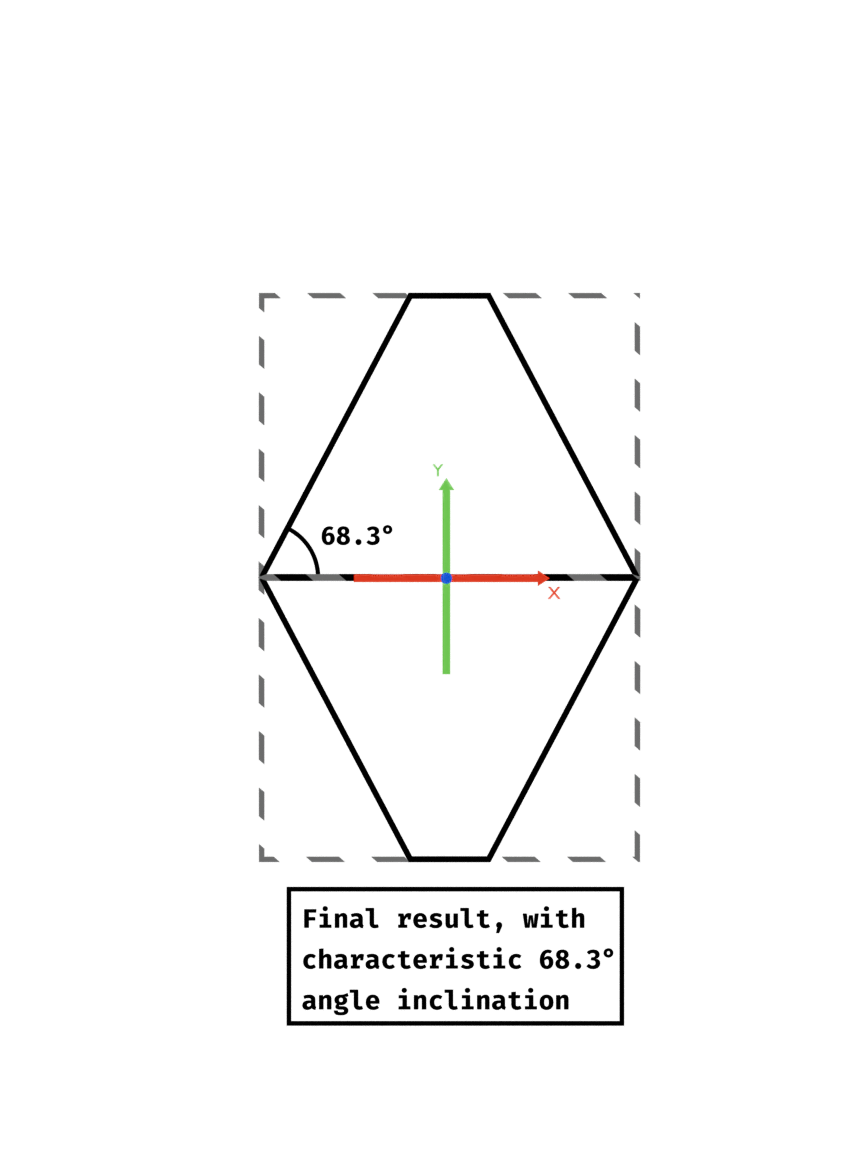
\includegraphics[width=.95\textwidth, clip]{./immagini/bipi_1_3.png}
        \caption{}
        \label{fig:bipyramids_process3}
    \end{subfigure}
    \caption{Creation steps: a) Scale along Y axis b) inset of the superior and inferior surfaces c) final standard model}
    \label{fig:bipyramids_process}
\end{figure}

\paragraph{Positioning process: }

After that, it must be positioned onto one of the diagonal faces, since the small bottom base will not ensure the maximum equilibrium. This is done by moving along the Y axis the model, so that the bottom base sits on the floor. Subsequently, a rotation matrix along the X axis is applied to rotate the bipyramid of $68.3^{\circ}$, as shown in Fig. \ref{fig:bipyramids_positioning}:

\begin{figure}[ht]
    \centering
    \begin{subfigure}[b]{0.22\textwidth}
        % bipi_2_1
        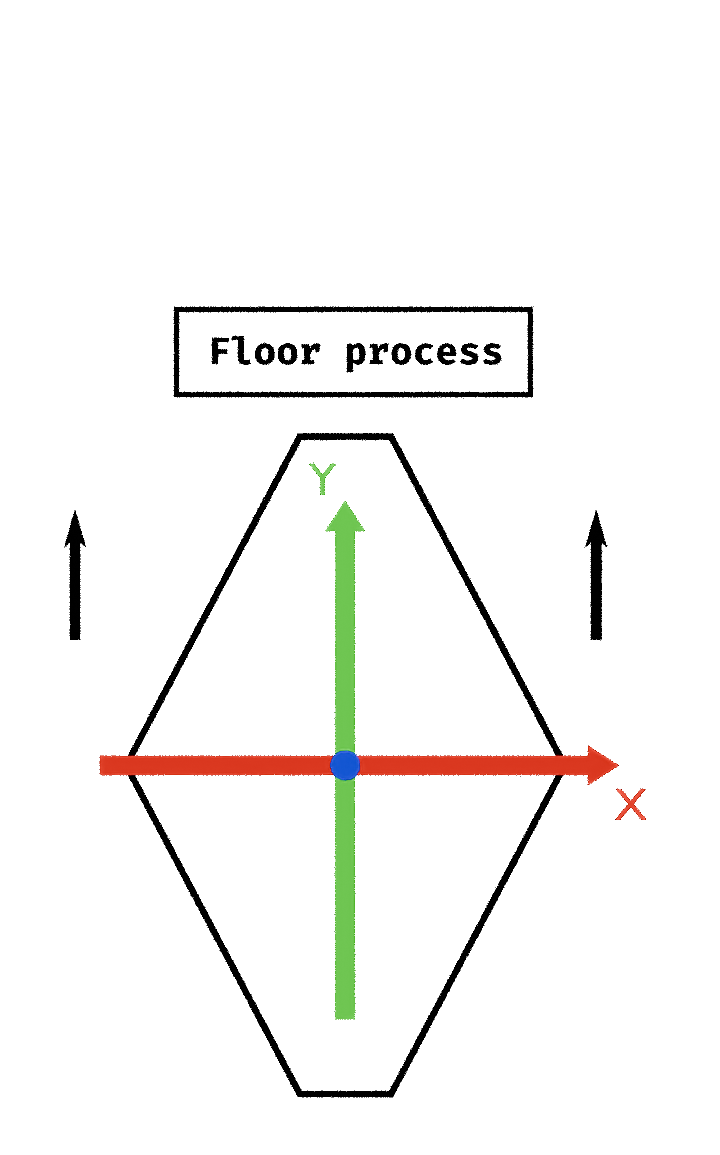
\includegraphics[width=.95\textwidth, clip]{./immagini/bipi_2_1.png}
        \caption{}
        \label{fig:bipyramids_positioning1}
    \end{subfigure}
    \hfill
    \begin{subfigure}[b]{0.22\textwidth}
        % bipi_2_2
        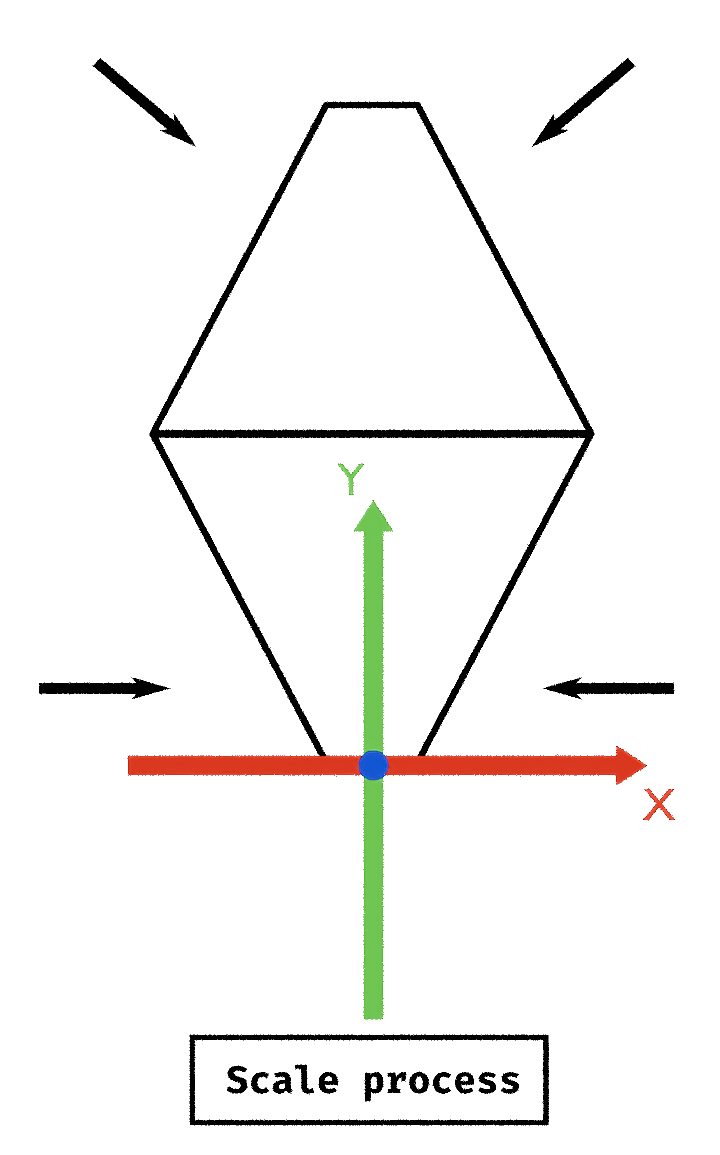
\includegraphics[width=.95\textwidth, clip]{./immagini/bipi_2_2.png}
        \caption{}
        \label{fig:bipyramids_positioning2}
    \end{subfigure}
    \hfill
    \begin{subfigure}[b]{0.22\textwidth}
        % bipi_2_3
        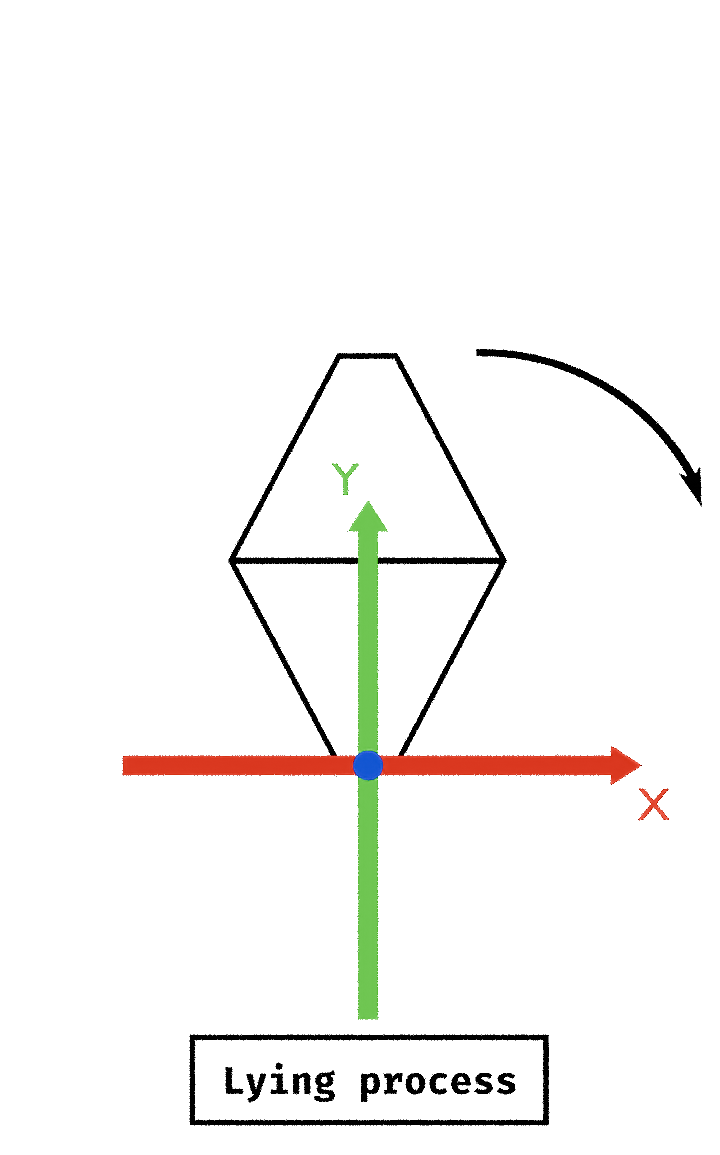
\includegraphics[width=.95\textwidth, clip]{./immagini/bipi_2_3.png}
        \caption{}
        \label{fig:bipyramids_positioning3}
    \end{subfigure}
    \hfill
    \begin{subfigure}[b]{0.22\textwidth}
        % bipi_2_4
        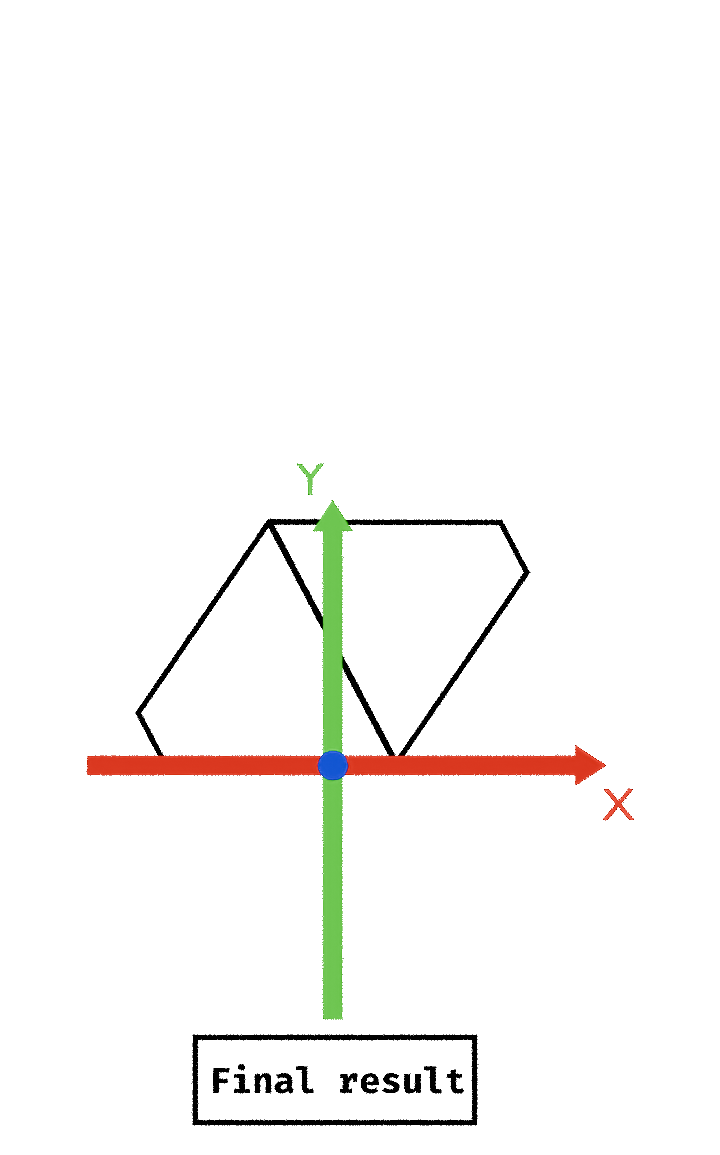
\includegraphics[width=.95\textwidth, clip]{./immagini/bipi_2_4.png}
        \caption{}
        \label{fig:bipyramids_positioning4}
    \end{subfigure}
    \caption{Instance positioning: a) floor process b) scaling process c) lying process d) final positioned model}
    \label{fig:bipyramids_positioning}
\end{figure}


\newpage

Finally, a traslation is applied in order to center the model on its center of mass. Thus, it will be easier for the user to position and rotate the desired nanoparticles on the substrate.

\paragraph{Examples: }

Some example of generated images are reported in Fig. \ref{fig:bipiramid_type} a-c. In particular, Fig. \ref{fig:bipiramid2} and \ref{fig:bipiramid3} shown also compenetrated nanosheets that are successfully handled by this system.

\begin{figure}[ht]
    \centering
    \begin{subfigure}[b]{0.3\textwidth}
        % bipiramid_singola
        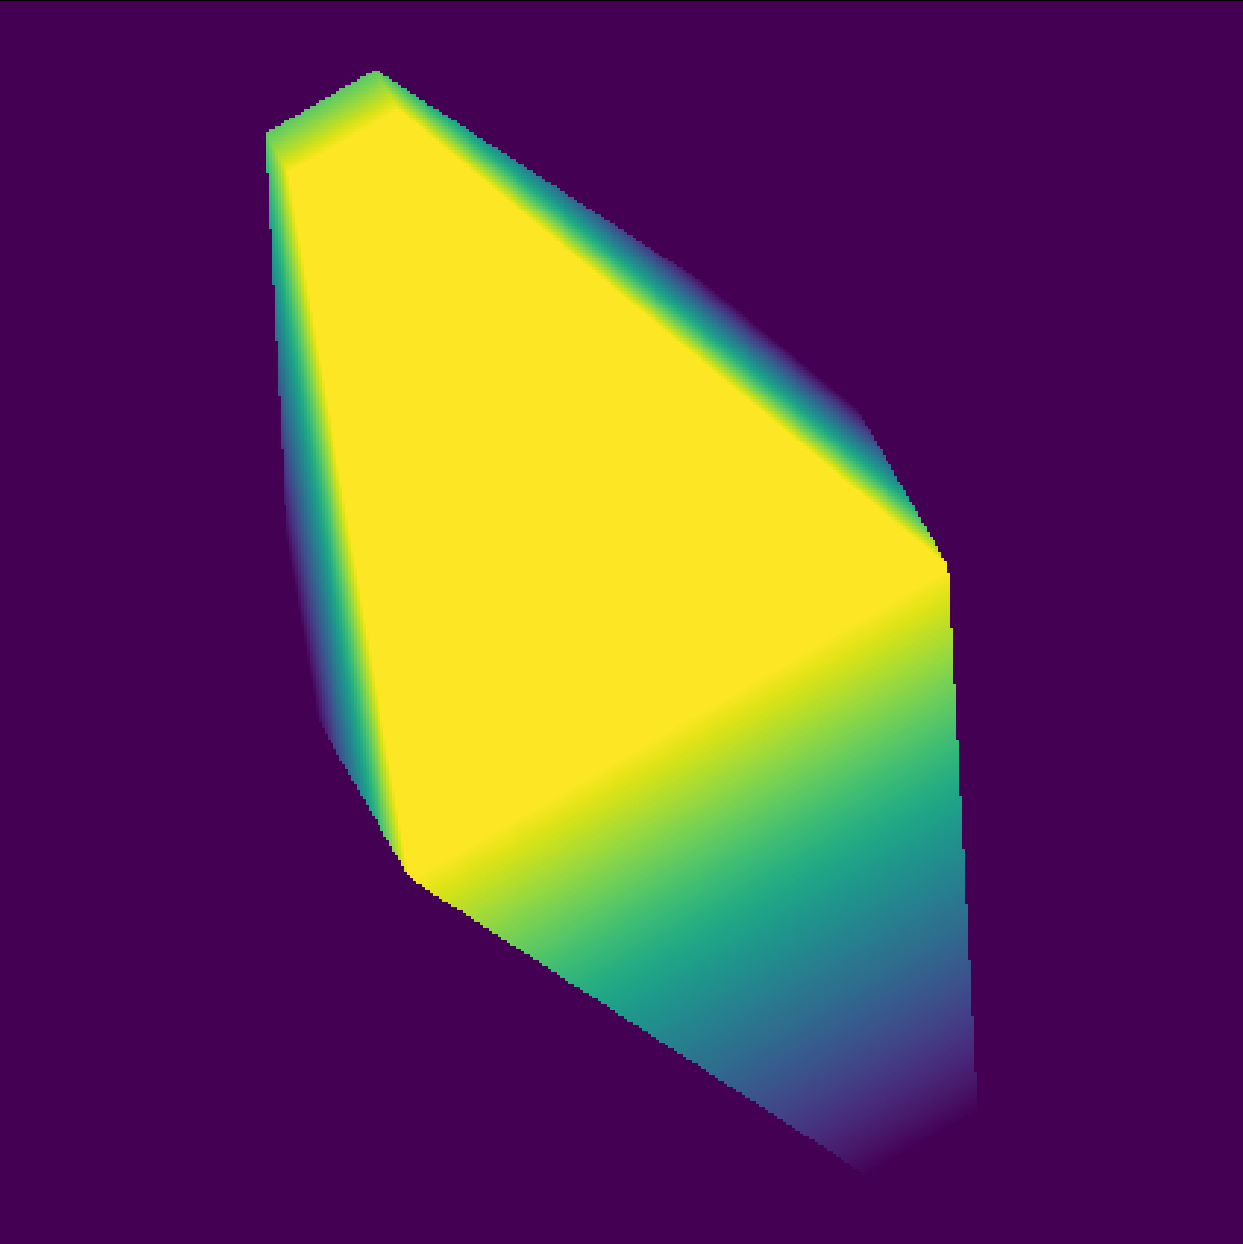
\includegraphics[width=.95\textwidth]{./immagini/bipiramid_singola.png}
        \caption{}
        \label{fig:bipiramid1}
    \end{subfigure}
    \hfill
    \begin{subfigure}[b]{0.3\textwidth}
        % bipiramid_doppia
        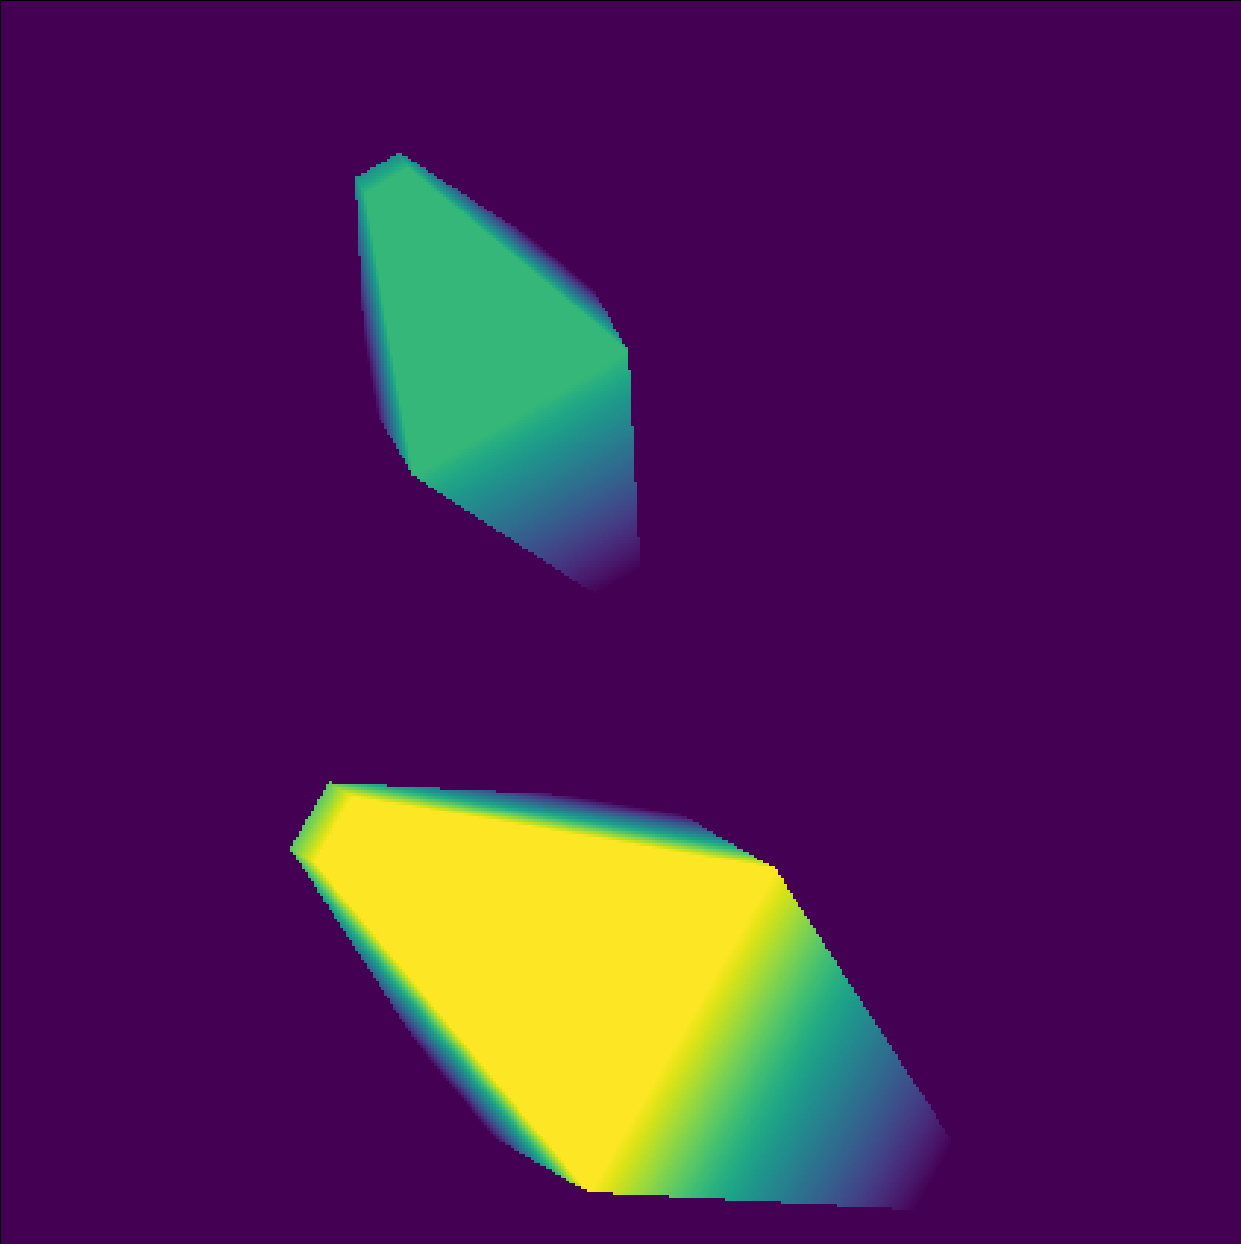
\includegraphics[width=.95\textwidth]{./immagini/bipiramid_doppia.png}
        \caption{}
        \label{fig:bipiramid2}
    \end{subfigure}
    \hfill
    \begin{subfigure}[b]{0.3\textwidth}
        % bipiramid_statistica
        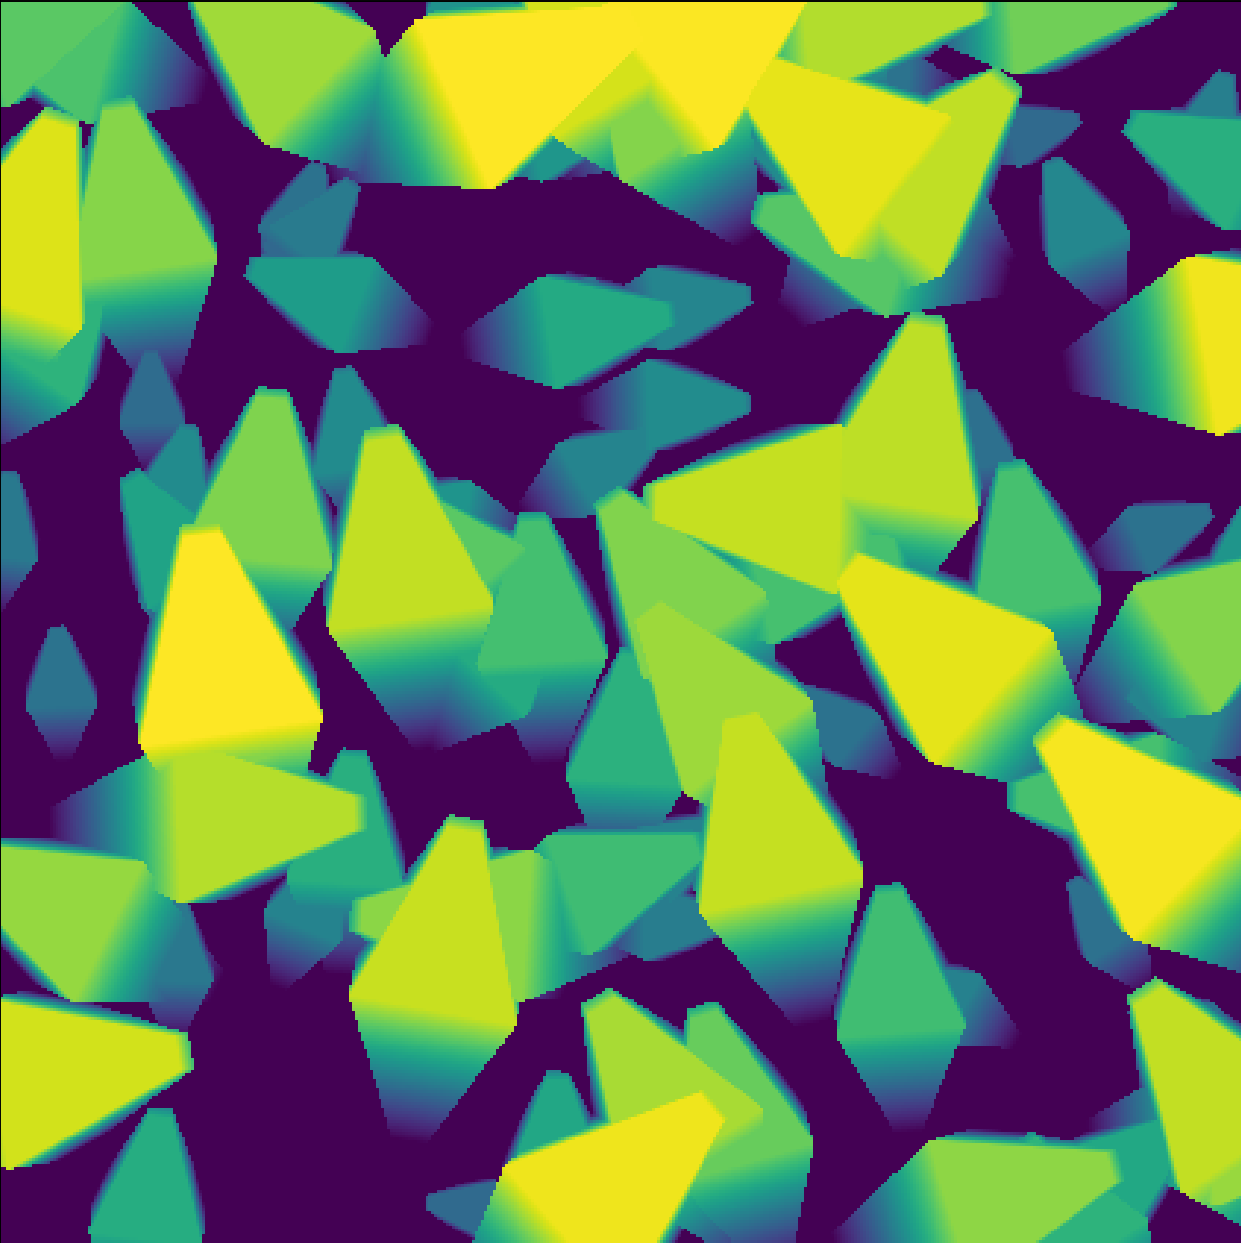
\includegraphics[width=.95\textwidth]{./immagini/bipiramid_statistica.png}
        \caption{}
        \label{fig:bipiramid3}
    \end{subfigure}
    \caption{Example of usage of bipiramids: a) Single b) Double c) Statistic}
    \label{fig:bipiramid_type}
\end{figure}

\chapter{Structure fitting}

\section{Maximum filter: working principle}

In order to automatize completely this method, the introduction of additional layers for the image recognition are required. In Fig. \ref{fig:local_max} the different steps are shown:

\begin{itemize}
    \item First of all some features must be extracted from a given raw image i.e. the local maxima, that indicate where the spherical nanoparticles are located.
    \item This approach fails in understanding which local maxima are fit for our structure generation. For this reason, a threshold is introduced to choose which of the found points are valid. In this work the threshold has been set equal to the nominal radius of the nanoparticle.
\end{itemize}

\begin{figure}[ht]
    \centering
    % filtro_max
    \includegraphics[width=.95\textwidth]{./immagini/filtro_max.png}
    \caption{Steps for image recognition: a) Raw image b) Extracted local maxima c) Threshold application}
    \label{fig:local_max}
\end{figure}

\section{Tip size estimation}

Once the peaks have been found, we can obtain from their height the size of the nanoparticle we will be building. Once we have all the informations, we can generate the structure that will be used as a kernel for our morphological filter.

\begin{figure}[ht]
    \centering
    \begin{subfigure}[b]{0.325\textwidth}
        % 2_labl
        \includegraphics[width=.98\textwidth, trim={30, 0, 30, 0}, clip]{./immagini/2_labl.png}
        \caption{}
        \label{fig:process_steps_a}
    \end{subfigure}
    \hfill
    \begin{subfigure}[b]{0.325\textwidth}
        % 5_labl
        \includegraphics[width=.98\textwidth, trim={30, 0, 30, 0}, clip]{./immagini/5_labl.png}
        \caption{}
        \label{fig:process_steps_b}
    \end{subfigure}
    \hfill
    \begin{subfigure}[b]{0.325\textwidth}
        % 3_labl
        \includegraphics[width=.98\textwidth, trim={30, 0, 30, 0}, clip]{./immagini/3_labl.png}
        \caption{}
        \label{fig:process_steps_c}
    \end{subfigure}
    \caption{Process steps: a) Raw image b) Found peaks c) Generated structures}
    \label{fig:process_steps}
\end{figure}


Before reconstructing the tip, we need to estimate the domain/size of the tip, which can be done using the previous maps. It will ensure a good resolution and a low computing time. Once the structures have been fitted under the topography, the tip matrix size must be estimated to cover the largest sample present in the image. However, in order to have an high resolution tip after the erosion process, it is important not to overestimate this parameter. In fact, the size of the convolution output matrix is determined by the difference in the number of pixels between the structure size and the original data size. Also the underestimating of the tip matrix size would be an issue, since the result would include only the tip apex with loss of tip sides.

To estimate the largest feature in the sample we approach the problem by creating a mask (Fig. \ref{fig:boolean_a}) able to select only the points with the height values greater than a given threshold. Therefore, to obtain the perimeter of the areas, the derivative calculation of the boolean mask is performed along X and Y direction (Fig. \ref{fig:boolean_b}).

\newpage

\begin{figure}[ht]
    \centering
    \begin{subfigure}[b]{0.45\textwidth}
        % maschera_picchi
        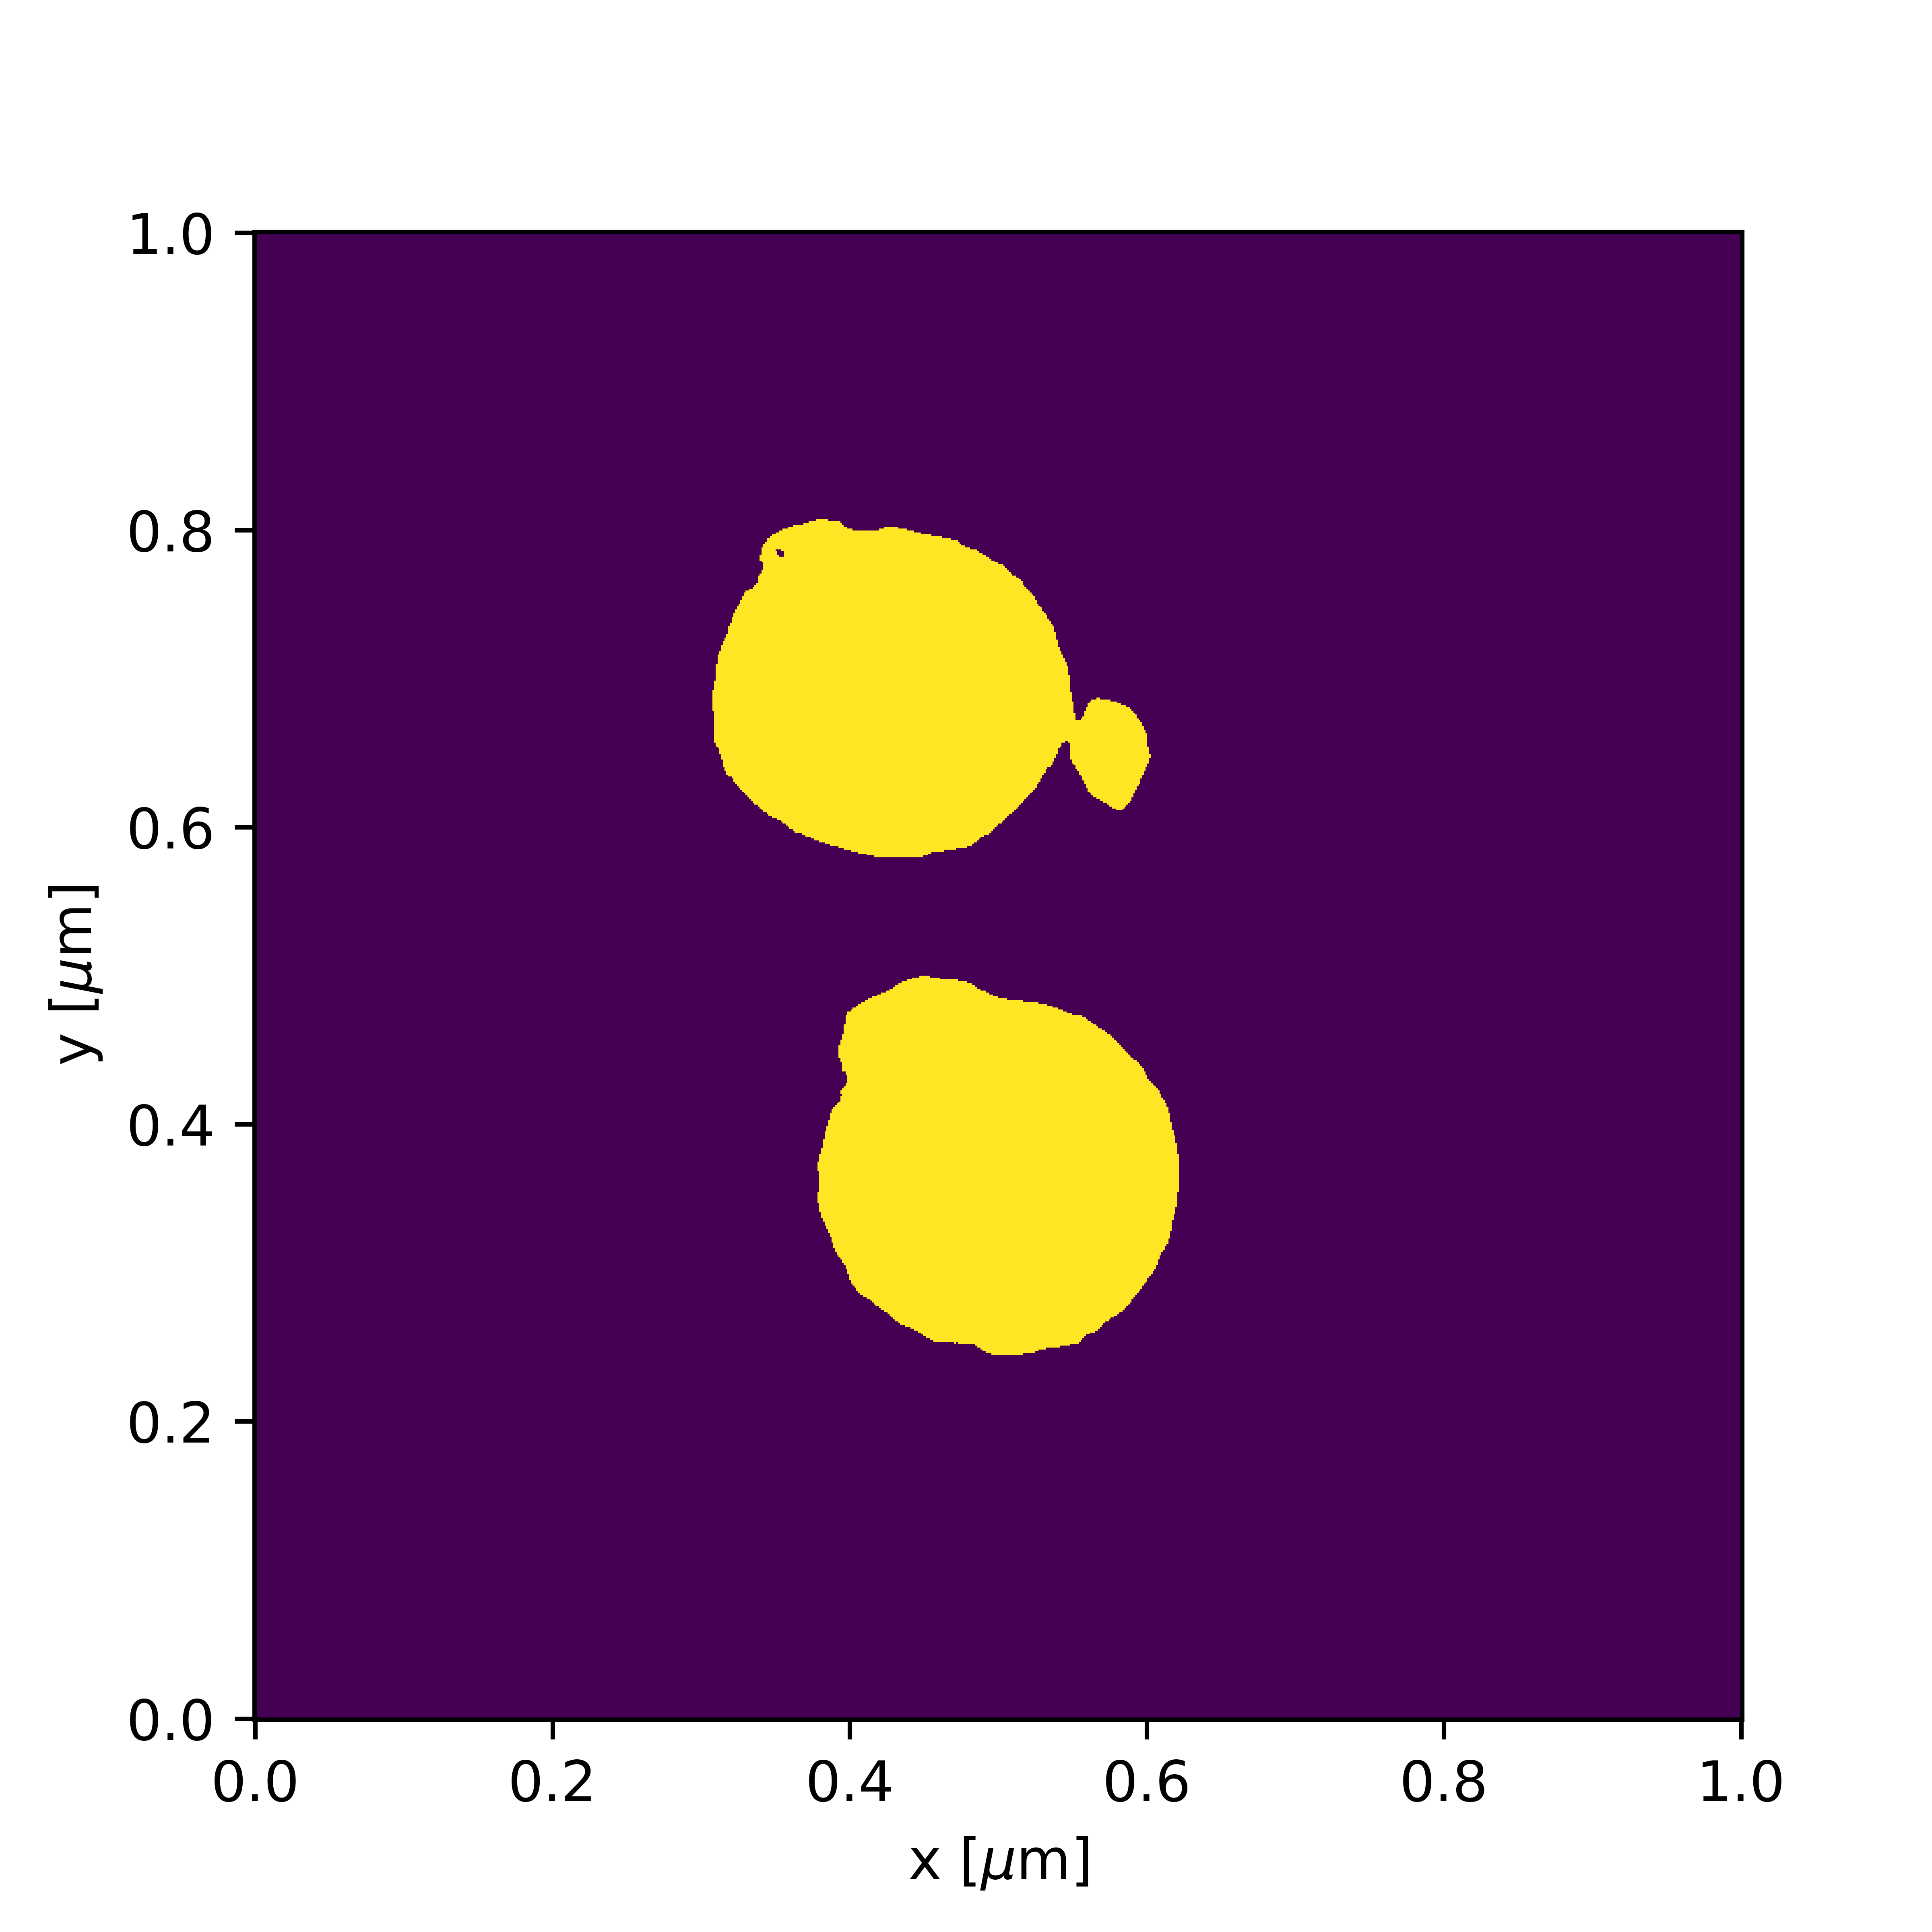
\includegraphics[width=.98\textwidth]{./immagini/maschera_picchi.png}
        \caption{}
        \label{fig:boolean_a}
    \end{subfigure}
    \hfill
    \begin{subfigure}[b]{0.45\textwidth}
        % derivatives
        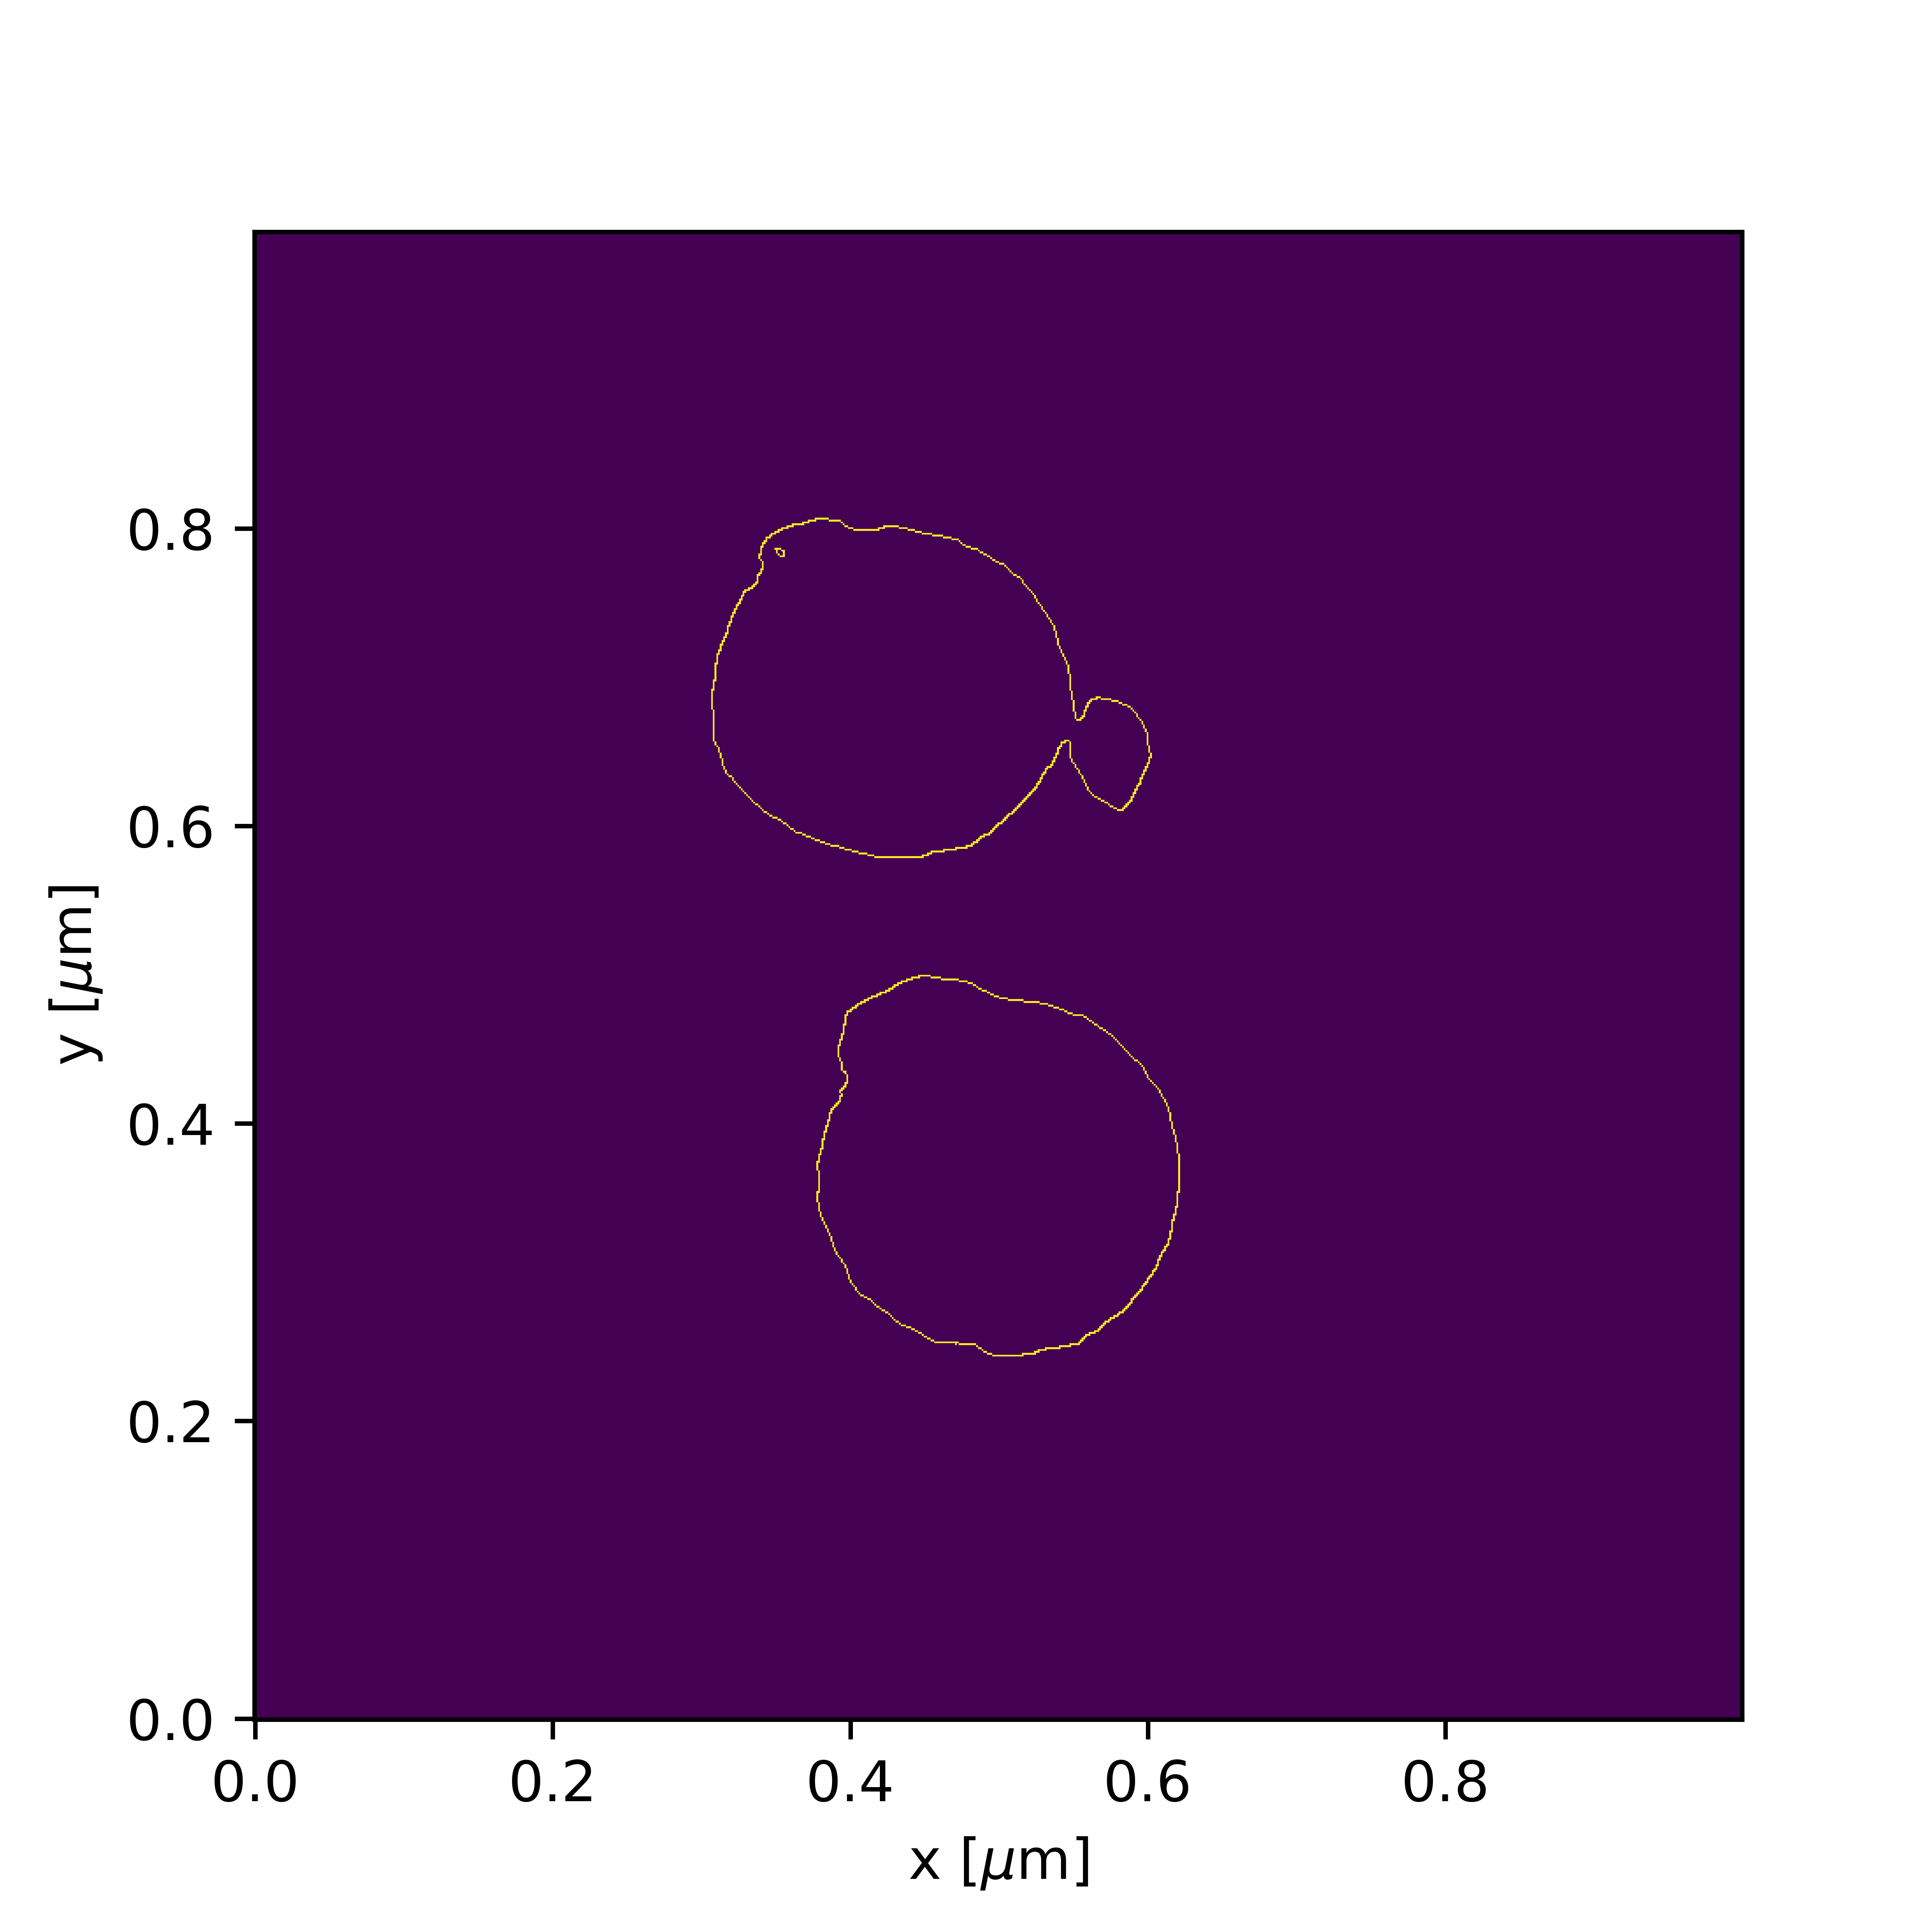
\includegraphics[width=.98\textwidth]{./immagini/derivatives.png}
        \caption{}
        \label{fig:boolean_b}
    \end{subfigure}
    \caption{a) mask, b)  binary derivation for Tip size estimation}
    \label{fig:boolean}
\end{figure}

It is known that the derivative of a boolean mask returns True if there's a change in the value of the data and False otherwise. Then, we scan line by line each in both directions and all the extracted True indices have been coupled. The difference of the elements in each couple represents the width of the feature between the two indices. The maximum value of this difference was finally used as a parameter to obtain the final tip matrix size, which will be increased by an additional radius (example: +10\%) to guarantee a border around the reconstructed tip.
\section{Tip reconstruction - image deconvolution}

\paragraph{Erosion algorithm: }

The erosion algorithm, as introduced by Villarubbia \cite{scanning_microscope,Villarrubia}, is aimed at reconstructing the tip shape based on both the actual and the ideal topography data. This algorithm, known as the naive erosion method, was initially devised to determine the covering envelope of a sphere as it moves across a surface. The envelope essentially represents the path traced by the center of the sphere as it rolls over the sampled points on the surface.

Notice that, although the structuring element in this specific implementation is a sphere, it is important to highlight, in a broader context, that this algorithm can be extended to many other shapes such as bipyramids, nanosheets, and more. When considering these alternative shapes, it becomes challenging to visualize how they would interact with the surface in a rolling motion. Therefore, it is more accurate to describe the interaction of the structuring element with the surface as a planar displacement rather than a rolling action.

\paragraph{Mathematical solution: }

The algorithm takes two key inputs: the surface to undergo erosion (denoted as S) and the structuring element (denoted as B). Then it applies the erosion equation (reflected in Equation \ref{eq:erosion}) to each pair of coordinates (u, v) within the topography data.

\begin{equation}
    \label{eq:erosion}
    T(x, y) = S \ominus B = \min_{u, v}\left(S(x + u, y + v) - B(u, v)\right)
\end{equation}

Basically, the naive erosion algorithm aligns with the principles of morphological dilation and erosion (as shown in Fig. \ref{fig:filter}), which are essentially defined as the Minkowski addition and subtraction operations \cite{erosion_Minkowskische} between the input set and the structuring element, respectively. This mathematical framework underpins the process of shape transformation and reconstruction within the context of the erosion algorithm.

\begin{figure}[ht]
    \centering
    \begin{subfigure}[b]{0.45\textwidth}
        \includegraphics[width=.98\textwidth]{./immagini/erosion2.png}
        \caption{}
        \label{fig:filter_a}
    \end{subfigure}
    \hfill
    \begin{subfigure}[b]{0.45\textwidth}
        \includegraphics[width=.98\textwidth]{./immagini/erosion3.png}
        \caption{}
        \label{fig:filter_b}
    \end{subfigure}
    \caption{Morphological filters (The structuring element is the apex tip): b) Dilation process on a sample profile c) Erosion process on a sample profile}
    \label{fig:filter}
\end{figure}

\newpage

In the following Fig. \ref{fig:confronto_pre_post} the original topography (a) and the deconvoluted result (b) of the naive erosion algorithm are shown.

\begin{figure}[ht]
    \centering
    \begin{subfigure}[b]{0.40\textwidth}
        % 2
        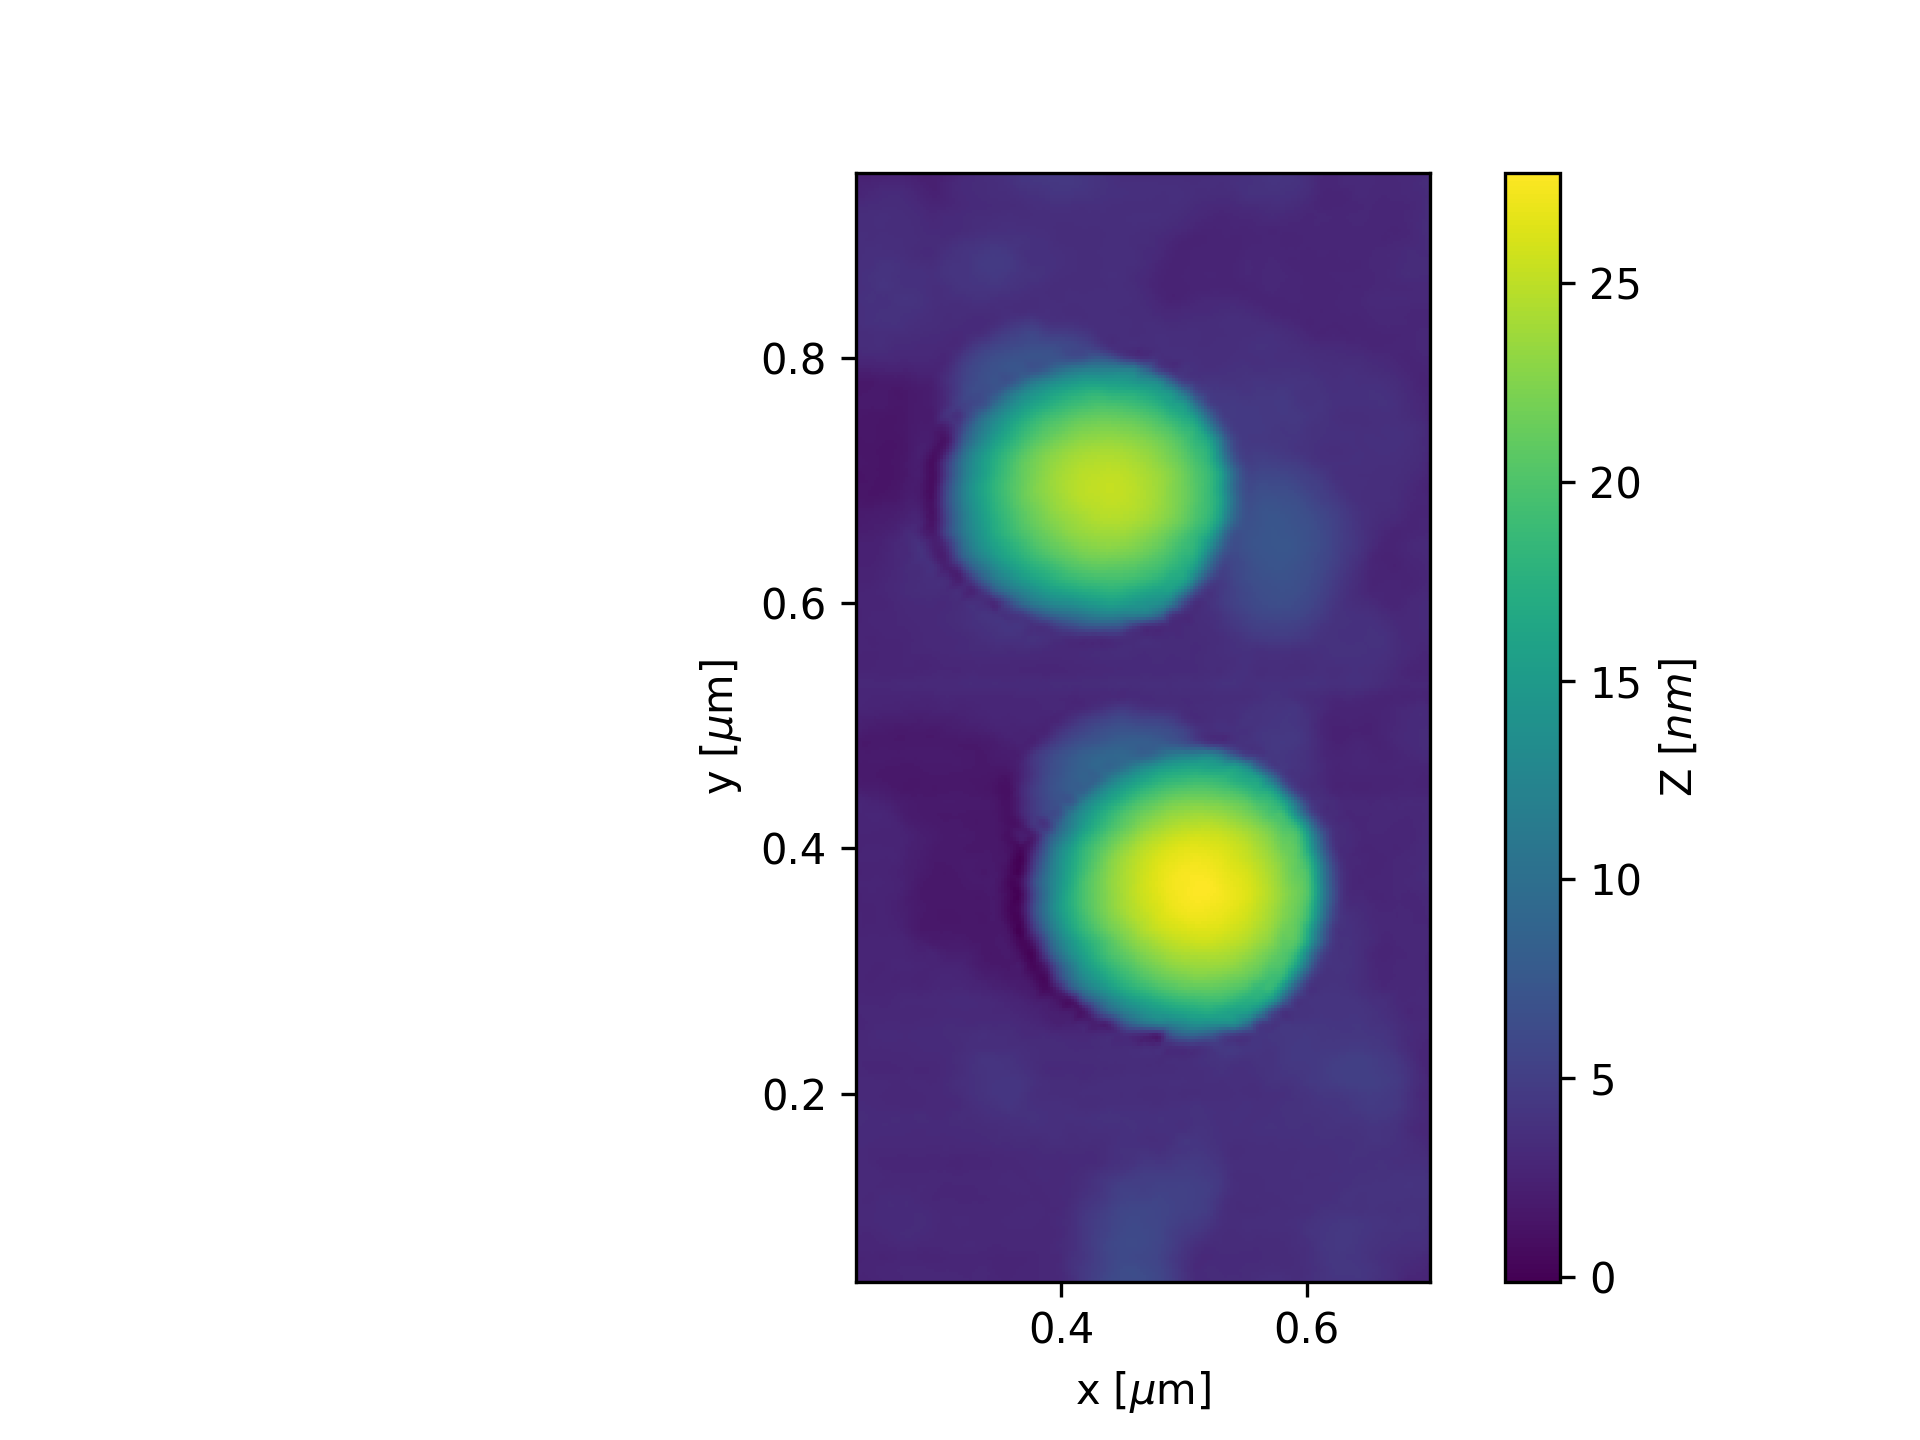
\includegraphics[width=.95\textwidth, trim={170, 0, 40, 0}, clip]{./immagini/2.png}
        \caption{}
        \label{fig:prima}
    \end{subfigure}
    \hfill
    \begin{subfigure}[b]{0.40\textwidth}
        % 4
        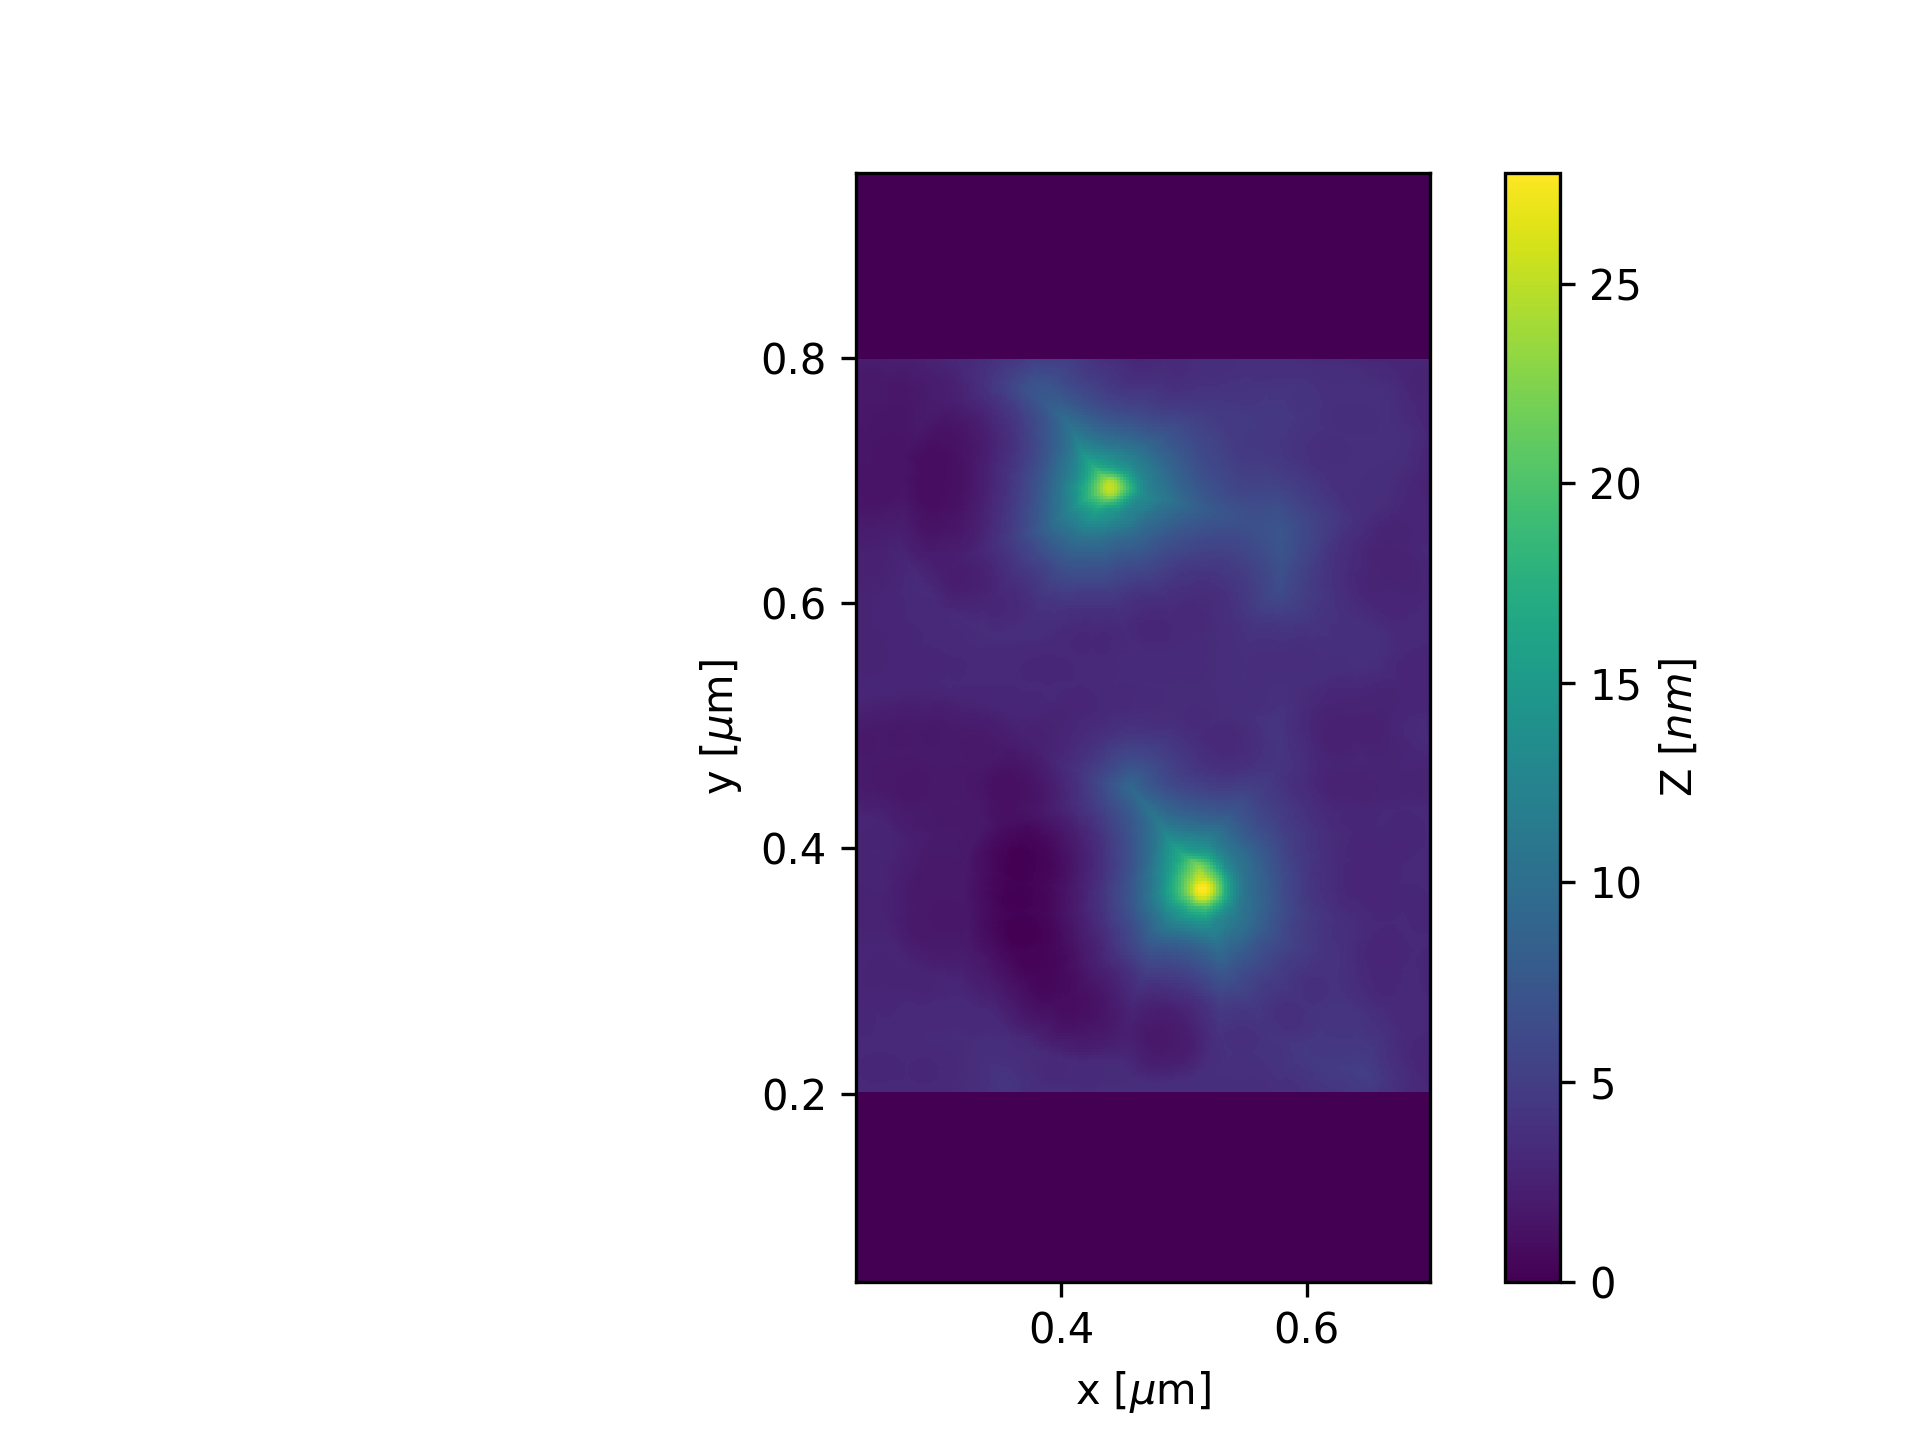
\includegraphics[width=.95\textwidth, trim={170, 0, 40, 0}, clip]{./immagini/4.png}
        \caption{}
        \label{fig:dopo}
    \end{subfigure}
    \caption{Results a) Original Data b) Deconvoluted image}
    \label{fig:confronto_pre_post}
\end{figure}

In Fig. \ref{fig:tiptredi}, the reconstructed tip, as obtained from just the Minkowski subtraction, is shown. 

\begin{figure}[ht]
    \centering
    % punta_finale
    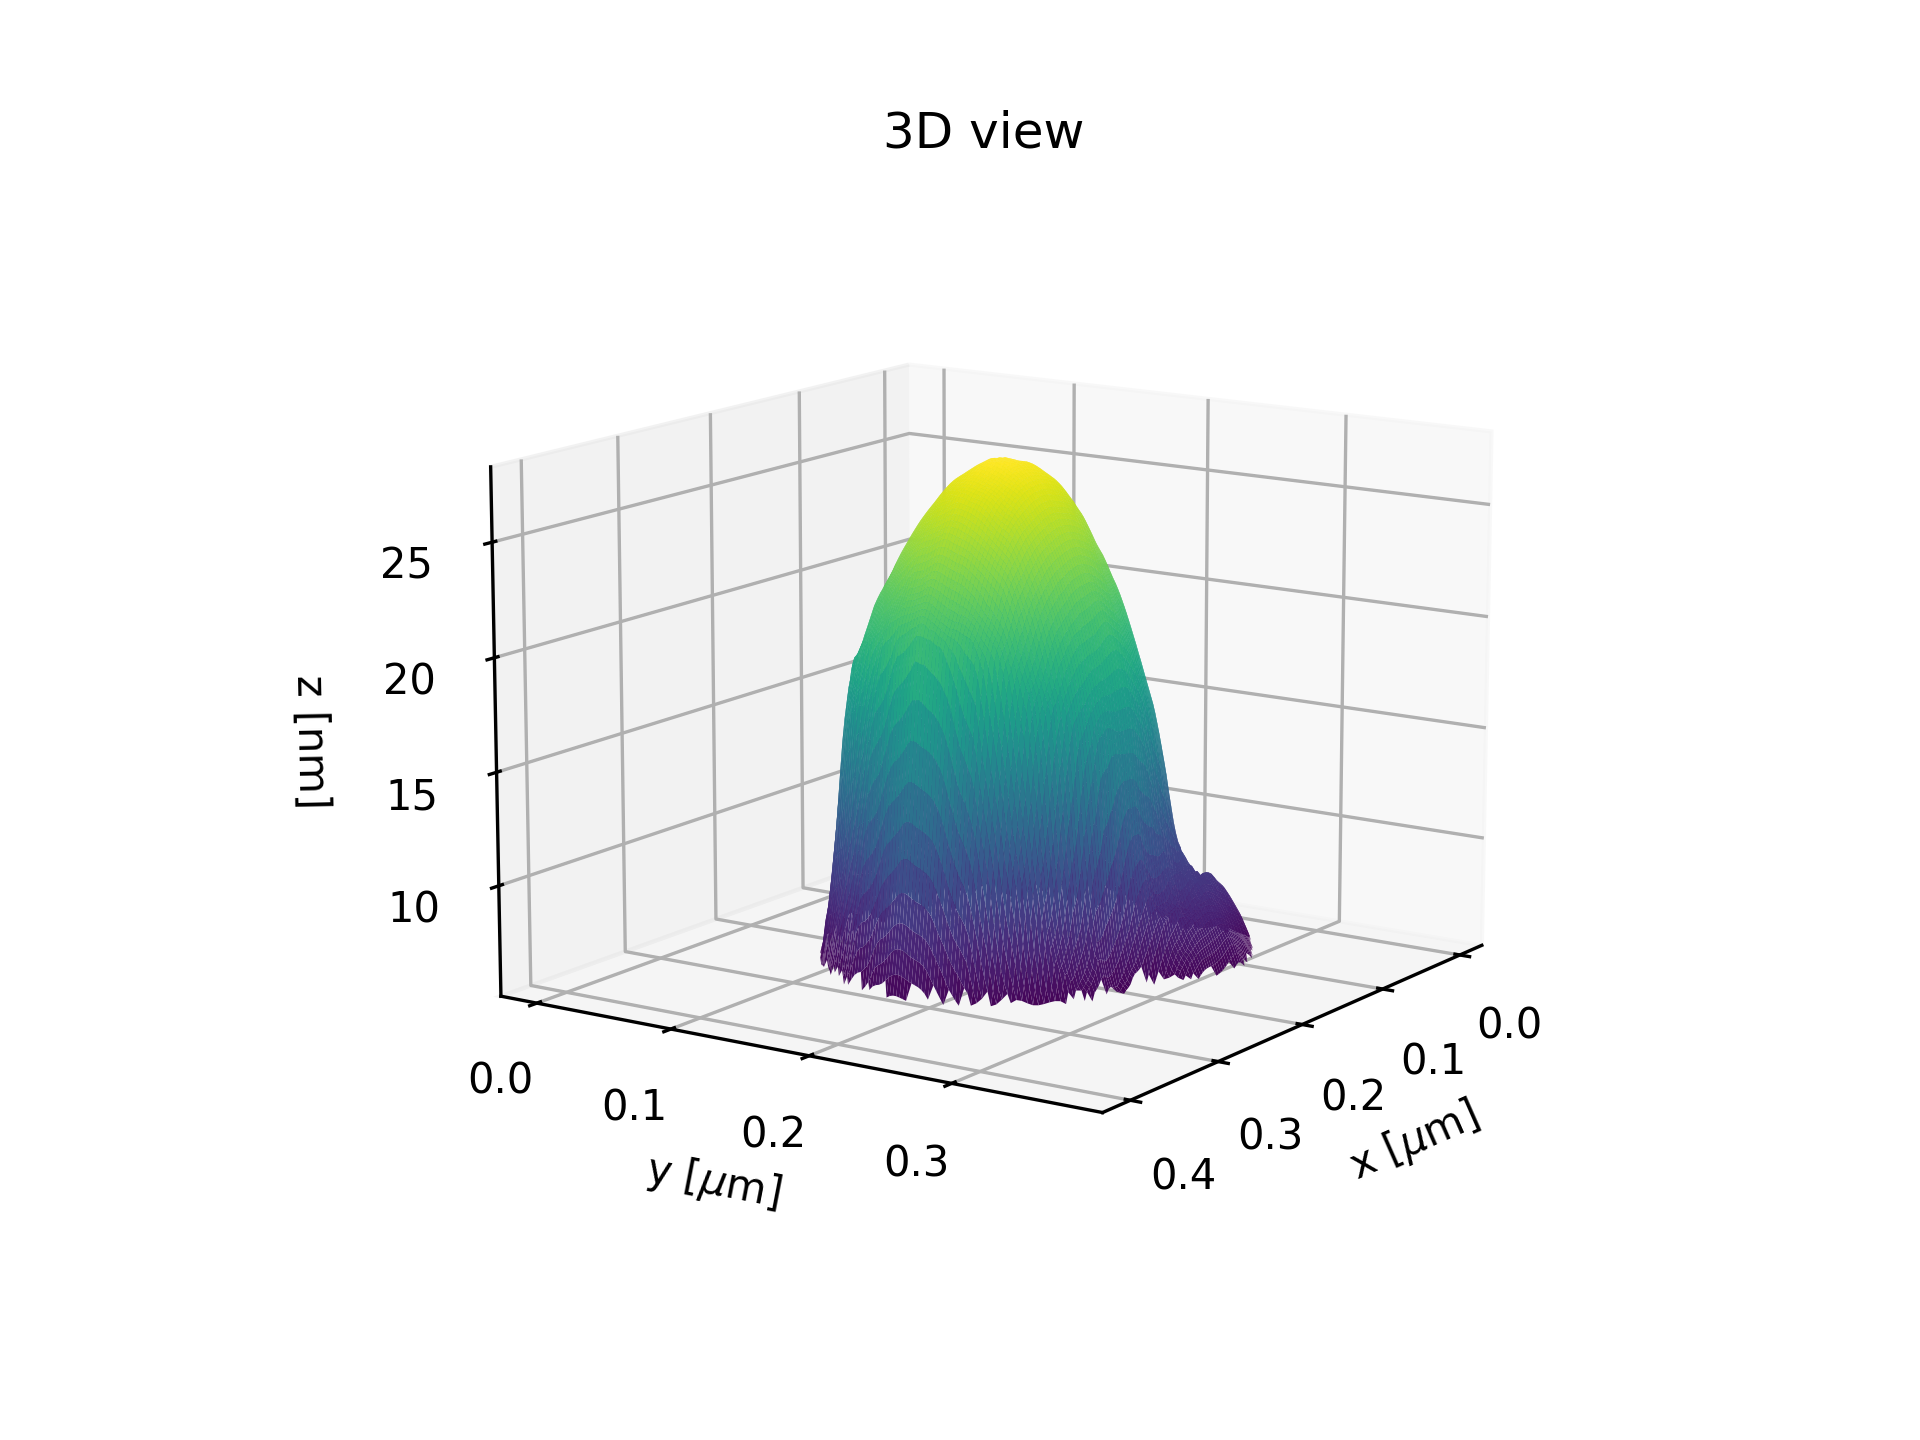
\includegraphics[width=.7\textwidth]{./immagini/punta_finale.png}
    \caption{Reconstructed 3D tip}
    \label{fig:tiptredi}
\end{figure}
\chapter{Conclusions}

The aim of this study was to reconstruct the tip shape via \textit{'ray tracer method'}, starting from the generation, via Python module, of the ideal topography of the tip characteriser. Then the tip shape reconstruction was made by “eroding” the real measurement with the generated structure.
More in detail, the \textit{ray tracer} approach allows to generate multiple models of the expected sizes and orientations, then to analyse them by means of image recognition algorithm and finally, to proceed with the eroding algorithm.

In particular in this work the complete implementation of a spherical support was performed, as a crucial starting point for the development of more complex structures. This means that, given the images of nanospheres, we can reconstruct AFM tips, which is the main step for the deconvolution of AFM topographies. The same approach can be easily scaled to other shapes, but at this time a full-automatic algorithm generates all the intermediate steps. Once the simulation is finished, it is possible to obtain statistics on how well the program performed compared to more established methods, thus providing insight into a further improvement.

In conclusion, we can state that the ability to simulate ideal measurements and accurately to reconstruct tip shapes using ray tracing techniques opens up new possibilities for improving the precision and speed of tip reconstruction algorithms in AFM studies. 

\vspace{10pt}

As a further perspective, studies on different tip shapes will benefit from the groundwork established by the sphere implementation. More in detail, we will focus on the $TiO_2$ nanosheets, that, due to their unique properties and challenging applications, are widely investigated in material science \cite{scarano}.


\fontsize{10}{12}\selectfont

\bibliographystyle{unsrt}
\addcontentsline{toc}{chapter}{\bibname}
\bibliography{thesis}  

\end{document}


% L'impaginazione dopo la correzione
% citazione bipiramidi e nanosheets